\documentclass[fleqn,10pt]{JLA_article}

\usepackage{array}
\usepackage{tabularx}
\usepackage{float}
\usepackage{longtable}
\usepackage{pdflscape}
\usepackage{placeins}
\usepackage{tikz}
\usetikzlibrary{arrows.meta,calc,positioning,shapes.geometric}
\hypersetup{hidelinks,breaklinks=true,pdftitle={Pathway-Centric Evaluation of Synthetic Educational Time-Series Data},pdfauthor={Anonymous}}

\PaperTitle{Pathway-Centric Evaluation of Synthetic Educational Time-Series Data}
\Authors{Anonymous author(s)}
\Keywords{synthetic data, learning analytics, educational trajectories, rare learner pathways, evaluation, privacy}
\Submitted{Under review}
\Accepted{}
\Published{}
\Volume{0}
\Number{0}
\Pages{1---14}
\Doi{TBD}

\Notesname{Notes for Practice}
\note{Synthetic educational data are often judged by aggregate similarity, although learning-analytics uses also depend on sequential structure and uncommon learner pathways that may matter for intervention.}
\note{Across the evaluated datasets and generators, matching overall patterns did not ensure realistic learning sequences or uncommon pathways. Standard synthetic-only training lowered mean overall next-step prediction in every tested combination; neither standard nor targeted augmentation improved that mean.}
\note{Before using or sharing synthetic learner records, check pathway frequencies and behavior, prediction on separate real learners, and possible disclosure of training records; emphasizing rare pathways is not an automatic correction.}

\Abstract{Learning analytics depends on detailed records of how learners interact, progress, struggle, and disengage over time. However, these records often contain sensitive information and can be difficult to share, limiting replication, benchmarking, and the development of learning-analytics models. In recent years, synthetic data have attracted growing attention in privacy-sensitive fields such as healthcare and finance, where access to real data is often restricted. Similar interest is emerging in education, where synthetic data can provide artificial learner records that resemble real data without directly distributing the original records.

Yet educational data pose a particular challenge: learner behavior unfolds over time. Reproducing overall statistics is therefore not enough. Important learning-analytics questions often concern uncommon patterns in learner sequences, which we call \emph{pathways}, such as persistent struggle, recovery, or late disengagement. If synthetic data distort or omit these pathways, researchers may build models or draw conclusions that appear valid overall but fail for the learners or situations that motivate intervention.

We address this gap by assessing \emph{pathway-level predictive usefulness}: how well models trained on synthetic learner trajectories predict outcomes for real learners following uncommon pathways. We also assess pathway prevalence and behavior among learners matching each pathway. We examine population patterns, temporal structure, pathway representation, and predictive performance on held-out real learners across multiple educational datasets and contrasting generation methods. We find that synthetic data that appear realistic overall can still distort learning processes and provide limited support for uncommon learner pathways. Standard synthetic-only training reduced mean overall next-step predictive performance in every tested dataset--generator combination; neither standard nor targeted augmentation improved mean overall next-step performance. Pathway-specific and additional learner-level results were mixed. Our study provides a practical approach for determining when synthetic educational data are fit for learning-analytics research.}

\emergencystretch=2em
% Layout-only: let floats use available space without changing JLA typography.
\setlength{\textfloatsep}{10pt plus 2pt minus 2pt}
\setlength{\floatsep}{8pt plus 2pt minus 2pt}
\setlength{\intextsep}{8pt plus 2pt minus 2pt}
\renewcommand{\topfraction}{0.9}
\renewcommand{\bottomfraction}{0.8}
\renewcommand{\textfraction}{0.08}
\renewcommand{\floatpagefraction}{0.9}
\setcounter{topnumber}{4}
\setcounter{bottomnumber}{3}
\setcounter{totalnumber}{5}
% Reduce heading whitespace; retain the class's heading fonts and labels.
\titlespacing*{\section}{0pc}{2ex plus 2pt minus 1pt}{5pt}
\titlespacing*{\subsection}{0pc}{1.5ex plus 2pt minus 1pt}{0pt}
\titlespacing*{\subsubsection}{0pc}{1.5ex plus 1pt minus 1pt}{0pt}
\titlespacing*{\paragraph}{0pc}{1ex plus 1pt minus 1pt}{10pt}
\widowpenalty=10000

\newcommand{\msd}[2]{\ensuremath{#1 \mathbin{\pm} #2}}
\newcommand{\msdn}[3]{\ensuremath{#1 \mathbin{\pm} #2_{\scriptscriptstyle n=#3}}}
\newcommand{\bmsd}[2]{\ensuremath{\mathbf{#1 \mathbin{\pm} #2}}}
\newcommand{\R}{\mathcal{R}}
\newcommand{\SYN}{\mathcal{S}}
\newcommand{\MAE}{\operatorname{MAE}}
\newcommand{\JS}{\operatorname{JS}}
\newcommand{\NMI}{\operatorname{NMI}}

\begin{document}

\raggedbottom
\maketitle
\thispagestyle{fancy}

\section{Introduction}

Learning analytics (LA) uses data on learners' responses and activities over time to study progress, struggle, and disengagement~\cite{siemens2013emergence,knight2017time,molenaar2014sequential}. Learner records are sensitive, and removing identifiers alone does not resolve disclosure concerns~\cite{slade2013ethics,liu2023understanding}. A \emph{learner trajectory} is one learner's sequence of responses or activities in a course or system. A \emph{synthetic trajectory} is a generated sequence of the same kind, based on patterns in real data. A \emph{pathway} is a behavioral pattern that multiple trajectories can share, such as recovery after early difficulty. Synthetic trajectories could support replication, benchmarking, and comparisons across instructional contexts without distributing the original learner records~\cite{haim2023openscience,gasevic2016context}. The value of synthetic trajectories depends on whether the generated records preserve the behavior needed for a particular analysis.

For example, the sequences \emph{incorrect, incorrect, correct, correct} and \emph{correct, correct, incorrect, incorrect} both have an overall correctness rate of 50\%. The first sequence suggests recovery from early difficulty, whereas the second suggests declining performance. Sequence, duration, and timing matter for understanding learning~\cite{knight2017time,molenaar2014sequential,saint2020combining}. A synthetic dataset can match aggregate rates of correctness or engagement while omitting, overproducing, or distorting pathways such as persistent struggle, recovery, and late disengagement. Misrepresented pathways can distort conclusions about learning processes and weaken predictions for real learners within those pathways.

Prior LA research has evaluated synthetic educational data through resemblance to real records, predictive utility, and disclosure risk~\cite{liu2024scaling,liu2025fairprivate}. Recent LAK work has also generated longitudinal learner sequences~\cite{huang2026pathways}. Aggregate-only evaluations, however, do not show whether an uncommon pathway occurs at a plausible rate, whether behavior within the pathway resembles real behavior, or whether models trained on synthetic data predict well for real learners who follow the pathway. Disclosure requires a separate audit because synthetic records can retain information about training learners~\cite{stadler2022synthetic,vanbreugel2023membership}.

The limits of aggregate-only evaluation motivate two research questions:

\begin{samepage}
\begin{enumerate}[label=\textbf{RQ\arabic*.}, leftmargin=*,topsep=4pt,itemsep=4pt,parsep=0pt]
    \item How well do synthetic trajectories reflect real learner behavior, including uncommon pathways?
    \item How does pathway targeting affect the representation of uncommon pathways and prediction for real learners, both overall and within those pathways?
\end{enumerate}
\end{samepage}

To address these questions, we use the \emph{Pathway-Centric Evaluation Lens}, which treats pathway representation and pathway-level prediction as central to judging synthetic-data quality, rather than relying on population averages alone. The lens checks how often responses and activities occur, how they unfold over time, whether uncommon pathways are represented, whether synthetic data support prediction, and whether training records might be exposed. RQ1 applies the first three checks to standard generation, which gives no extra weight to any pathway. In RQ2, pathway-targeted generation gives more weight to training learners whose trajectories match uncommon pathway rules. Disclosure is audited separately.

We assess pathway prevalence, behavior within each pathway group, and prediction for held-out real learners who follow each pathway. We call the prediction check \emph{pathway-level predictive usefulness}, extending train-on-synthetic/test-on-real evaluation~\cite{esteban2017realvalued,yoon2019timegan,flanagan2022fine} from the full test population to uncommon pathways. A \emph{rare pathway} is a pattern matched by only a small share of trajectories under a stated dataset-specific rule. The term \emph{rare} describes a pattern of activity, not a learner identity or an assumed need for intervention. Pathway rules classify complete trajectories into retrospective evaluation groups. Predictors use only earlier behavior and known task context; no predictor receives pathway membership as an input.

We compare Markov, a sequence variational autoencoder (SeqVAE), and TimeGAN on ASSISTments, EdNet KT1, and weekly OULAD. Pathway rules are estimated from real training learners, and prediction is evaluated on separate real test learners. Across three ASSISTments runs, SeqVAE's synthetic data differed from real training data by a mean of only 0.12 percentage points in overall correctness. Across the same runs, a pathway defined by unusual skill ordering appeared in an average of 98.52\% of synthetic learners, compared with 4.87\% of real training learners. Our contribution is an evaluation protocol that connects population and temporal checks to pathway representation and predictive usefulness for real learners (Table~\ref{tab:evaluation-lens}).
% Keep explanatory paragraphs intact when floats move to a page boundary.
\interlinepenalty=10000

Table~\ref{tab:evaluation-lens} is a roadmap from each research question to the comparisons used to answer it and the corresponding Results section. Disclosure appears separately because it is a supporting audit, not a third research question.

\begin{table}[!htbp]
\centering
\caption{Study roadmap: the comparisons used to answer each research question and where the results appear.}
\label{tab:evaluation-lens}
\label{tab:rq-design}
\small
\setlength{\tabcolsep}{4pt}
\renewcommand{\arraystretch}{1.15}
\begin{tabularx}{\linewidth}{|>{\raggedright\arraybackslash}p{3.4cm}|>{\raggedright\arraybackslash}X|>{\raggedright\arraybackslash}p{2.4cm}|}
\hline
Question or audit & Comparison & Results \\ \hline
RQ1\newline Reflecting real behavior & Compare standard synthetic trajectories with real training trajectories: response and activity rates, event order and timing, and the frequency and within-group behavior of uncommon pathways. & Section~\ref{sec:rq1-results} \\ \hline
RQ2\newline Effect of targeting & Compare standard and targeted synthetic trajectories against real training data for pathway representation. Train predictors on real data, synthetic data, or both; test all predictors on the same held-out real learners, overall and within uncommon pathways. & Section~\ref{sec:rq2-results} \\ \hline
Separate audit\newline Disclosure & Check standard and targeted synthetic trajectories for close copying of real training trajectories and signals revealing who was in the training set. & Section~\ref{sec:disclosure-results} \\ \hline
\end{tabularx}
\end{table}
\FloatBarrier

\section{Methodology}

Figure~\ref{fig:pipeline} summarizes the study. In the tutoring datasets, each trajectory is a sequence of attempts; in OULAD, each trajectory tracks weekly activity for one course enrollment. A pathway rule groups trajectories that share a behavioral pattern, such as recovery after early difficulty.

A \emph{generator} creates synthetic trajectories from patterns in real training records; a \emph{predictor} estimates an educational outcome from recorded history and known context. We assess synthetic resemblance against real training data (RQ1) and prediction on separate real test learners (RQ2). Standard and pathway-targeted generation produce matching numbers of learners and records.

We combine established measures of distributional similarity, temporal dependence, detectability, prediction, and membership inference~\cite{lin1991divergence,strehl2002cluster,lopezpaz2017c2st,davis2006precision,fawcett2006roc,saito2015precision,shokri2017membership} with a pathway-level prediction check. Pathway rules, thresholds, and minimum counts are benchmark choices, not universal standards; the Supplementary Material gives complete calculation rules and results.


\subsection{Data, Temporal Units, and Learner Separation}

The benchmark uses ordered tutoring attempts from ASSISTments 2009--2010 Skill Builder~\cite{feng2009assistments} (3{,}429 training / 788 test trajectories), question-answering attempts from EdNet KT1~\cite{choi2020ednet} (7{,}703 / 1{,}963), and weekly course engagement from the Open University Learning Analytics Dataset (OULAD)~\cite{kuzilek2017oulad} (26{,}072 / 6{,}521). Each OULAD trajectory is a course enrollment with one record per observed week. The supplement gives record and variable counts; Table~\ref{tab:prediction-specification} specifies the prediction tasks.

We use a nominal 80/20 \emph{learner-disjoint split}: each learner's records belong entirely to training or test data. In OULAD, all enrollments of the same student remain together. This prevents \emph{data leakage}, or unintended use of test-learner information in model development.

Preprocessing assigns consistent category codes and numerical intervals (\emph{bins}). All data-dependent transformations are estimated using real training data and applied unchanged to synthetic and test data. Prediction inputs contain prior behavior and known task context, not the response or activity being predicted; the first event is excluded because it has no history.

\begin{figure}[!htbp]
\centering
% Native vector icons and source tags keep the figure editable and legible in
% grayscale. Repeated tags replace long, crossing reuse arrows.
\begingroup
\definecolor{pipeink}{HTML}{243547}
\definecolor{pipemuted}{HTML}{586675}
\definecolor{pipeblue}{HTML}{28658C}
\definecolor{pipeteal}{HTML}{187A72}
\definecolor{pipepurple}{HTML}{70549A}
\definecolor{pipemagenta}{HTML}{9B527B}
\definecolor{pipegold}{HTML}{916817}
\definecolor{pipeslate}{HTML}{58677E}
\colorlet{pipeR}{pipeblue}
\colorlet{pipeF}{pipeteal}
\colorlet{pipeH}{pipegold}
\colorlet{pipeS}{pipepurple}
\colorlet{pipeT}{pipemagenta}
\hyphenpenalty=10000
\newcommand{\pipetag}[1]{\textcolor{pipe#1}{\textbf{[#1]}}}

% #1 name, #2 x, #3 y, #4 width, #5 height, #6 color,
% #7 icon, #8 heading, #9 body. All process cards share one grid.
\newcommand{\pipeprocess}[9]{%
    \node[process, draw=#6!45, fill=#6!5,
        minimum width=#4cm, minimum height=#5cm] (#1) at (#2,#3) {};
    \fill[#6!13] ($(#1.north west)+(0.40,-0.37)$) circle (0.25cm);
    \pic[draw=#6] at ($(#1.north west)+(0.40,-0.37)$) {#7};
    \node[processtitle, text width={#4cm-1.03cm}]
        at ($(#1.north west)+(0.82,-0.22)$) {#8};
    \node[processbody, text width={#4cm-0.48cm}]
        at ($(#1.north west)+(0.24,-0.68)$) {#9};
}
\newcommand{\pipestage}[4]{%
    \fill[#3, rounded corners=3pt] (0,#1-0.31) rectangle (17.2,#1+0.31);
    \node[font=\fontencoding{T1}\sffamily\bfseries\fontsize{9}{10}\selectfont,
        text=white, inner sep=0pt] at (0.43,#1) {#2};
    \draw[white!45!#3, line width=0.5pt] (0.86,#1-0.17) -- (0.86,#1+0.17);
    \node[stage] at (1.10,#1) {#4};
}
% #1 x, #2 top y, #3 color, #4 icon, #5 title, #6 dimension label.
\newcommand{\pipeeval}[6]{%
    \draw[draw=#3!40, fill=white, rounded corners=3pt, line width=0.6pt]
        (#1,#2) rectangle (#1+8.4,#2-3.61);
    \fill[#3!9, rounded corners=3pt]
        (#1+0.015,#2-0.015) rectangle (#1+8.385,#2-1.04);
    \fill[#3!17] (#1+0.48,#2-0.48) circle (0.29cm);
    \pic[draw=#3, scale=1.12] at (#1+0.48,#2-0.48) {#4};
    \node[cardtitle, text=#3] at (#1+0.98,#2-0.22) {#5};
    \node[dim] at (#1+0.98,#2-0.66) {#6};
}

\begin{tikzpicture}[
    x=1cm, y=1cm, text=pipeink,
    font=\fontencoding{T1}\sffamily\fontsize{8.5}{10.5}\selectfont,
    process/.style={line width=0.6pt, rounded corners=3pt,
        inner sep=0pt, outer sep=0pt},
    processtitle/.style={anchor=north west, inner sep=0pt, align=left,
        font=\fontencoding{T1}\sffamily\bfseries\fontsize{8.5}{10}\selectfont},
    processbody/.style={anchor=north west, inner sep=0pt, align=left,
        font=\fontencoding{T1}\sffamily\fontsize{8.3}{10.2}\selectfont},
    flow/.style={draw=pipemuted!85, line width=0.85pt,
        -{Stealth[length=1.7mm,width=1.3mm]}, shorten <=1.5pt, shorten >=1.5pt},
    stage/.style={anchor=west, inner sep=0pt, text=white,
        font=\fontencoding{T1}\sffamily\bfseries\fontsize{10}{12}\selectfont},
    detail/.style={anchor=west, inner sep=0pt, text=pipemuted,
        font=\fontencoding{T1}\sffamily\fontsize{8}{10}\selectfont},
    cardtitle/.style={anchor=north west, inner sep=0pt, text width=7.08cm,
        font=\fontencoding{T1}\sffamily\bfseries\fontsize{9}{11}\selectfont},
    cardbody/.style={anchor=north west, inner sep=0pt,
        align=left, text width=7.80cm},
    dim/.style={anchor=north west, inner sep=0pt, text=pipemuted,
        font=\fontencoding{T1}\sffamily\fontsize{8}{10}\selectfont},
    % Consistent line icons, drawn natively rather than using an icon font.
    every pic/.style={line width=0.75pt, line cap=round, line join=round},
    pics/database/.style={code={
        \draw (-0.16,0.11) -- (-0.16,-0.12)
            arc[start angle=180,end angle=360,x radius=0.16,y radius=0.055]
            -- (0.16,0.11);
        \draw (0,0.11) ellipse[x radius=0.16,y radius=0.055];
        \draw (-0.16,-0.005)
            arc[start angle=180,end angle=360,x radius=0.16,y radius=0.055];
    }},
    pics/sequence/.style={code={
        \draw (-0.18,-0.09) -- (-0.02,0.11) -- (0.17,-0.04);
        \draw[fill=white] (-0.18,-0.09) circle (0.04);
        \draw[fill=white] (-0.02,0.11) circle (0.04);
        \draw[fill=white] (0.17,-0.04) circle (0.04);
    }},
    pics/split/.style={code={
        \draw (0,0.16) -- (0,0.03);
        \draw (-0.15,-0.14) -- (-0.15,0.03) -- (0.15,0.03) -- (0.15,-0.14);
        \draw (-0.20,-0.08) -- (-0.15,-0.14) -- (-0.10,-0.08);
        \draw (0.10,-0.08) -- (0.15,-0.14) -- (0.20,-0.08);
    }},
    pics/learners/.style={code={
        \draw (0,0.105) circle (0.065);
        \draw (-0.105,-0.16) -- (-0.105,-0.10)
            .. controls (-0.105,0.005) and (0.105,0.005) .. (0.105,-0.10)
            -- (0.105,-0.16) -- cycle;
        \draw (-0.16,0.065) arc[start angle=90,end angle=265,radius=0.05];
        \draw (0.16,0.065) arc[start angle=90,end angle=-85,radius=0.05];
    }},
    pics/lock/.style={code={
        \draw[rounded corners=0.5pt] (-0.14,-0.16) rectangle (0.14,0.055);
        \draw (-0.08,0.055) -- (-0.08,0.12)
            arc[start angle=180,end angle=0,radius=0.08] -- (0.08,0.055);
        \draw (0,-0.025) -- (0,-0.095);
    }},
    pics/check/.style={code={
        \draw (0,0) circle (0.17);
        \draw (-0.095,0) -- (-0.025,-0.07) -- (0.10,0.08);
    }},
    pics/target/.style={code={
        \draw (0,0) circle (0.17);
        \draw (0,0) circle (0.09);
        \draw (0,0) -- (0.18,0.18);
        \draw (0.11,0.18) -- (0.18,0.18) -- (0.18,0.11);
    }},
    pics/model/.style={code={
        \draw (-0.14,0.13) -- (0.14,0.10) -- (-0.14,-0.13)
            -- (0.14,-0.10) -- (-0.14,0.13);
        \foreach \x/\y in {-0.14/0.13,-0.14/-0.13,0.14/0.10,0.14/-0.10}
            \draw[fill=white] (\x,\y) circle (0.045);
    }},
    pics/synthetic/.style={code={
        \draw[rounded corners=0.5pt] (-0.15,-0.16) rectangle (0.09,0.12);
        \draw (-0.09,-0.08) -- (0.03,-0.08);
        \draw (-0.09,-0.01) -- (0.03,-0.01);
        \draw (0.14,0.035) -- (0.14,0.195);
        \draw (0.06,0.115) -- (0.22,0.115);
    }},
    pics/chart/.style={code={
        \draw (-0.17,0.16) -- (-0.17,-0.16) -- (0.18,-0.16);
        \draw (-0.11,-0.10) -- (-0.01,0.015) -- (0.07,-0.025) -- (0.17,0.14);
        \draw[densely dotted] (-0.11,-0.025) -- (-0.01,0.065)
            -- (0.07,0.035) -- (0.17,0.095);
    }},
    pics/branches/.style={code={
        \draw (-0.17,0) -- (-0.03,0) -- (0.12,0.13) -- (0.19,0.13);
        \draw (-0.03,0) -- (0.12,-0.13) -- (0.19,-0.13);
        \draw[fill=white] (-0.17,0) circle (0.035);
        \draw[fill=white] (0.19,0.13) circle (0.035);
        \draw[fill=white] (0.19,-0.13) circle (0.035);
    }},
    pics/shield/.style={code={
        \draw (0,0.18) -- (0.16,0.11) -- (0.14,-0.045)
            .. controls (0.12,-0.12) and (0.055,-0.16) .. (0,-0.19)
            .. controls (-0.055,-0.16) and (-0.12,-0.12) .. (-0.14,-0.045)
            -- (-0.16,0.11) -- cycle;
        \draw (-0.07,0.015) -- (-0.015,-0.04) -- (0.075,0.06);
    }},
    pics/settings/.style={code={
        \draw (-0.17,0.11) -- (0.17,0.11);
        \draw (-0.17,-0.02) -- (0.17,-0.02);
        \draw (-0.17,-0.15) -- (0.17,-0.15);
        \draw[fill=white] (-0.06,0.11) circle (0.04);
        \draw[fill=white] (0.08,-0.02) circle (0.04);
        \draw[fill=white] (-0.025,-0.15) circle (0.04);
    }}
]

% Compact overview: details remain in the methods and merged lens table.
\pipestage{13.00}{01}{pipeblue}{Separate learners before fitting rules or models}
\pipeprocess{raw}{2.60}{11.70}{5.20}{1.80}{pipeblue}{database}
    {Ordered learner trajectories}{ASSISTments, EdNet KT1, OULAD\\Learner-disjoint 80/20 split}
\pipeprocess{real}{8.50}{11.70}{5.60}{1.80}{pipeblue}{learners}
    {\pipetag{R} Real training learners}{Estimate processing rules and\\\pipetag{F} fixed pathway rules}
\pipeprocess{test}{14.50}{11.70}{5.40}{1.80}{pipegold}{check}
    {\pipetag{H} Held-out real learners}{Evaluation only; all enrollments of an OULAD student stay together}
\draw[flow] (raw.east) -- (real.west);
\draw[flow] (raw.south) -- (2.60,10.55) -- (14.50,10.55) -- (test.south);

\pipestage{9.97}{02}{pipepurple}{Generate matched datasets for each dataset, generator, and seed}
\pipeprocess{standardinput}{3.10}{8.69}{6.20}{1.70}{pipeblue}{learners}
    {Standard input: \pipetag{R}}{All learners have weight 1}
\pipeprocess{standardout}{12.00}{8.69}{10.40}{1.70}{pipepurple}{synthetic}
    {Fit generator $\rightarrow$ \pipetag{S} standard synthetic data}
    {Markov, SeqVAE, or TimeGAN\\Generate learner trajectories}
\draw[flow, draw=pipepurple!85] (standardinput) -- (standardout);
\pipeprocess{targetinput}{3.10}{6.72}{6.20}{1.85}{pipemagenta}{target}
    {Targeted input: \pipetag{R} with \pipetag{F}}
    {Eligible pathway union: weight 3\\Other learners: weight 1\\Overlapping rules do not compound}
\pipeprocess{targetout}{12.00}{6.72}{10.40}{1.85}{pipemagenta}{model}
    {Fit same generator family $\rightarrow$ \pipetag{T} targeted data}
    {All real-training learners remain eligible\\Same neural training-update limit as standard\\Matched seed and learner/record totals}
\draw[flow, draw=pipemagenta!85] (targetinput) -- (targetout);
\node[processbody, text width=17.0cm, text=pipemuted] at (0.10,5.57)
    {Shared processing: lengths estimated from \pipetag{R}; common normalization; OULAD profiles and terminal outcomes assigned after generation (Section~\ref{sec:generator-inputs}).};

\pipestage{4.57}{03}{pipeteal}{Evaluate preservation, predictive usefulness, and disclosure separately}
\pipeprocess{preserve}{2.75}{2.16}{5.50}{3.85}{pipeblue}{chart}
    {RQ1: Preservation}
    {Compare \pipetag{S} with \pipetag{R}: population composition and temporal processes.\\[4pt]
    Apply \pipetag{F} unchanged to compare pathway prevalence and within-pathway behavior.}
\pipeprocess{predict}{8.60}{2.16}{5.70}{3.85}{pipepurple}{target}
    {RQ2: Pathway-level prediction}
    {Fit predictors on \pipetag{R}, \pipetag{S}, \pipetag{R}+\pipetag{S}, \pipetag{T}, \pipetag{R}+\pipetag{T}; test on \pipetag{H}.\\[4pt]
    Apply \pipetag{F} to \pipetag{H} after prediction to score pathways; rules are not inputs.\\[4pt]
    Interpret with \pipetag{S}/\pipetag{T} pathway errors against \pipetag{R}.}
\pipeprocess{audit}{14.45}{2.16}{5.50}{3.85}{pipeslate}{shield}
    {Supporting disclosure audit}
    {Copying: \pipetag{S}/\pipetag{T} versus \pipetag{R}.\\[4pt]
    Membership: \pipetag{R} vs.\ \pipetag{H} using proximity to \pipetag{S}/\pipetag{T}, where applicable.\\[4pt]
    OULAD: exact copying in the activity/engagement projection only.}

\end{tikzpicture}
\endgroup

\vspace{2pt}
\caption{Leakage-safe benchmark pipeline. Tags identify reused data; ``+'' means training-data augmentation. [S] and [T] are finalized after shared processing. Pathway-level predictive usefulness is assessed on [H], with representation assessed against [R]. The same predictor settings apply to all five primary-task conditions; additional learner-level tasks use four (Section~\ref{sec:outcome-prediction}).}
\label{fig:pipeline}
\end{figure}

\subsection{Generator Inputs, Outputs, and Comparison}
\label{sec:generator-inputs}

The data tables supplied to the generators contain the relevant behavior, event type, assistance, timing, and course variables. Learner identifiers and event order mark sequence boundaries but are not values the generator learns to reproduce. Fields determined by other generated values, such as question metadata, are rebuilt after generation.

We compare three generators. An \emph{order-2 Markov/n-gram model} generates events from short recent histories, treating each event's attributes jointly. A \emph{sequence variational autoencoder} (SeqVAE)~\cite{kingma2014autoencoding} learns compact representations of short sequences and generates new sequences from the learned representations. \emph{TimeGAN}~\cite{yoon2019timegan}, implemented through SynthCity~\cite{qian2023synthcity}, learns temporal relationships using feedback from a second model that tries to distinguish real from generated sequences.

SeqVAE and TimeGAN train on \emph{windows}, or consecutive sections containing 20 observations. Standard and targeted conditions have the same maximum number of model updates, so targeting receives no additional training. This shared limit does not establish best achievable performance.

All generators share a real-training-estimated length procedure, adjusted to the required learner and record totals; individual learners' lengths are not directly resampled. Length measures therefore assess this shared procedure, not generator differences. Neural trajectories concatenate independently generated windows and truncate the last to the sampled length, without modeling continuity across window boundaries.

In OULAD, shared postprocessing assigns learner profiles through independent field-wise samples from real training data, conditional on course where available, and constructs end-of-course outcomes using a procedure estimated from real training data. Terminal outcomes are never generator inputs. Demographic resemblance therefore does not rank generators, and OULAD outcome tasks evaluate the complete generation-and-processing procedure, not direct outcome generation. The supplement details the OULAD profile-assignment and outcome-construction procedures.

Each dataset--generator combination uses three fixed random seeds, which control the random choices in each run. Test performance never determines generator or predictor settings or pathway cutoffs; Section~\ref{sec:uncertainty} describes uncertainty reporting.

\subsection{Pathway Definitions and Pathway-Targeted Training}

Pathway rules describe complete trajectories, such as low early correctness followed by recovery. The rules define retrospective evaluation groups, not information available for earlier prediction; separate early-history tasks predict later outcomes using only early observations (Section~\ref{sec:outcome-prediction}).

Rules are prespecified, with data-dependent thresholds estimated from real training data and applied unchanged to all four sources: real training, real test, standard synthetic, and targeted synthetic. \emph{Prevalence} is the proportion of trajectories satisfying a rule. Recomputing a lowest-5\% cutoff separately in each source would conceal frequency distortions.

Distribution-based rarity rules target the outer 5\% of real training data, with a 10\% ceiling to accommodate ties from binning. A pathway is unavailable if no nonempty real-training group meets this ceiling. Fixed thresholds distinguish changes between ordered trajectory halves; minimum lengths avoid single-event or empty-half classifications (Table~\ref{tab:rare-definitions}). Binned variables use their specified interval values. The supplement gives boundary conventions and exclusions.

\begin{table}[!htbp]
\centering
\caption{Pathway definitions used in the comparisons. Percentile cutoffs and the transition model are estimated using real training data and kept fixed for synthetic and test data.}
\label{tab:rare-definitions}
\small
\begin{tabular}{>{\raggedright\arraybackslash}p{0.29\linewidth}p{0.64\linewidth}}
\toprule
Pathway & Rule for identifying a trajectory \\
\midrule
Persistent low correctness / disengagement & Bottom 5\% whole-trajectory correctness or engagement and at least three observations. \\
Recovery / reengagement & First-half correctness or engagement at most 35\%, second-half rate at least 65\%, and at least four observations. \\
Late correctness decline / disengagement & First-half correctness or engagement at least 65\%, second-half rate at most 35\%, and at least four observations. \\
Rare skill / activity path & Unusual ordering of skills or activities: successive changes have low probability under a model estimated from real training data. Bottom 5\% of the resulting trajectory scores, with at least one transition; the exact calculation is in the supplement. \\
High hint use & Top 5\% whole-trajectory hints per attempt and at least three interactions; unavailable without varying hint use. \\
Rapid low-accuracy responding & Bottom 5\% mean response time, whole-trajectory correctness at most 50\%, and at least three interactions; an approximate behavioral indicator, not a validated diagnosis; unavailable without response time. \\
Long inactivity & Top 5\% maximum within-learner response- or inactivity-gap signal and at least three observations; unavailable without a declared gap signal. \\
\bottomrule
\end{tabular}
\end{table}

Targeted generator training assigns weight 3 to learners satisfying any eligible pathway rule and weight 1 otherwise; overlapping rules do not compound, and all learners remain eligible. This fixed emphasis is not tuned to datasets, generators, pathways, seeds, or results. Matched conditions retain generator family, learner/record totals, and neural training limit. Because pathways are emphasized together, changes do not isolate the causal effect of targeting one pathway. Selected groups and sizes are in the supplement.

\subsection{RQ-Aligned Evaluation Design}

Table~\ref{tab:rq-design} summarizes the comparisons. RQ1 uses standard synthetic data only: targeted data are excluded from its ranking because targeting deliberately changes the training distribution. RQ2 compares matched standard and targeted conditions, using real training data for representation checks and unchanged real test learners for prediction.

Comparisons follow available variables: correctness and skill in ASSISTments/EdNet, engagement and activity in OULAD, plus selected relationships, assistance, and timing measures. Supporting subgroup analyses compare subsequent behavior in groups defined from the first two observations using real-training-estimated rules.

\emph{Behavior-rate error} is the absolute difference between the real and synthetic proportions of correct responses or engaged weeks; zero indicates matching proportions. \emph{Three-event sequence divergence} compares the frequencies of three consecutive skills or activities; the implemented score ranges from 0 to 1, with zero indicating matching distributions. \emph{Trajectory-shape error} compares average behavioral development after aligning each trajectory to ten relative positions from beginning to end. We also calculate it separately within pathways; lower error indicates closer agreement.

For \emph{real-versus-synthetic detectability}, a separate histogram-based gradient-boosting model~\cite{friedman2001greedy} learns to identify each record's source and is tested on different learners. This method successively fits decision trees, or branching prediction rules, using binned numerical inputs. The detector predicts source, not an educational outcome: AUROC near 0.5 indicates chance-level separation, while larger values indicate more detectable differences. This direction differs from outcome-prediction AUROC, where larger values are desirable.

OULAD full-record detectability is excluded because independently assigned profiles and constructed outcomes prevent a fair comparison of the generators themselves. Only computationally costly diagnostics use reduced samples; generator training, pathway evaluation, and primary prediction tasks use their full specified data.

\subsection{Outcome Prediction and Pathway-Level Predictive Usefulness}
\label{sec:outcome-prediction}

Primary tasks predict next-response correctness in ASSISTments/EdNet and next-week engagement in OULAD; correctness or engagement is the positive outcome (value 1). A rare pathway need not have a rare positive outcome. OULAD engagement means a registered week with nonzero clicks, measuring platform activity rather than cognitive or emotional engagement.

We compare five predictor-training conditions: real only, standard synthetic only, real plus standard synthetic, targeted synthetic only, and real plus targeted synthetic. Synthetic-only conditions test replacement; combined conditions test \emph{augmentation}, or adding synthetic records to real training data. All use the same prespecified histogram-based gradient-boosting predictor settings and real test learners. Synthetic-only predictors use no real outcome records for fitting, but retain the common transformations estimated from real training data.

Table~\ref{tab:prediction-specification} specifies the implemented inputs, history lengths, outcomes, and count requirements. Previous values refer to the immediately preceding observation; cumulative quantities summarize only earlier observations. Task context (such as the question being attempted) can be known before its outcome.

% Verified against experiments/evaluation/{general_evaluation,learner_tasks,outcome_tasks}.py
% and per-seed downstream_utility_models.feature_columns in the source run reports.
\begin{table}[!htbp]
\centering
\caption{Implemented prediction tasks. Inputs exclude future behavior, terminal labels, and whole-trajectory pathway membership. Primary tasks use all prior observations (at least one). Minimum counts are calculation rules, not reliability guarantees.}
\label{tab:prediction-specification}
\footnotesize
\setlength{\tabcolsep}{3pt}
\begin{tabularx}{\linewidth}{@{}>{\raggedright\arraybackslash}p{2.15cm}>{\raggedright\arraybackslash}X>{\raggedright\arraybackslash}p{2.85cm}>{\raggedright\arraybackslash}p{3.8cm}@{}}
\toprule
Task / dataset & Predictor inputs and early-history windows & Positive outcome & Minimum counts / eligibility \\
\midrule
Next response: ASSISTments & Current skill; interaction index; previous correctness; cumulative correct count, interaction count, and correct rate; previous attempt, hint, response-time, and opportunity bins. & Correct next response. & Primary-task rules below; pathway counts refer to learners. \\
\addlinespace
Next response: EdNet & Current skill, question, and part; interaction index; previous correctness and part; cumulative correct count, interaction count, and correct rate; previous elapsed-time and timestamp-gap bins. & Correct next response. & Primary-task rules below; pathway counts refer to learners. \\
\addlinespace
Next week: OULAD & Course; week index; previous dominant activity, engagement, registration, click bin, active-days bin, and gap bin; cumulative engagement count, week count, and engagement rate. & Registered week with nonzero clicks. & Primary-task rules below; pathway counts refer to course enrollments. \\
\addlinespace
Later low correctness / recovery: tutoring datasets & First 2 attempts, with at least 2 later attempts: early correct rate, hint-use rate, mean attempt-bin value, distinct skill count, first skill, and mean response-time-bin value when available. Absent hint/attempt signals are zero constants. & Later correct rate at or below the real-training low-correctness cutoff; recovery: later rate at least 65\%. & At least 10 positive and 10 negative learners in each real train/test set. Recovery requires early correct rate at most 35\%. \\
\addlinespace
Later dropout / course failure: OULAD & First 4 weeks: course; engagement rate and last engagement; first and last dominant activity; distinct activity count; last gap bin. & Subsequent dropout; course failure among non-dropouts. & At least 10 positive and 10 negative enrollments in each real train/test set. Dropout requires registration throughout the first 4 weeks; failure excludes dropouts. \\
\bottomrule
\end{tabularx}
\par\smallskip\raggedright
Primary-task rules: nonempty train/test sets and both outcome classes for fitting and ranking. Within-pathway publication additionally requires 10 real test learners (or OULAD enrollments), not 10 per outcome class.
\end{table}


Our primary measure is \emph{area under the precision--recall curve} (AUPRC)~\cite{davis2006precision,saito2015precision}. It summarizes the trade-off between precision (the fraction of predicted positives that actually have the positive outcome) and recall (the fraction of actual positives identified) across cutoffs. We prioritize it because outcome frequencies can be unequal, including within pathways. Higher values indicate better prediction on the same sample; the test sample's positive-outcome proportion provides the no-skill reference. We also report \emph{area under the receiver operating characteristic curve} (AUROC), which measures how well positives rank above negatives~\cite{fawcett2006roc}. Higher outcome AUROC is better.

Each eligible next response or next week contributes one prediction to the score, so longer trajectories contribute more predictions. The uncertainty calculation keeps each learner's predictions together, but does not give all learners equal weight in the reported score.

For pathway-level predictive usefulness, we score existing real-test predictions within groups subsequently identified by the fixed pathway rules; membership is not a predictor input. Four differences measure replacement loss (real only minus standard synthetic only), standard augmentation gain (real plus standard minus real only), targeted replacement gain (targeted synthetic only minus standard synthetic only), and targeted augmentation gain (real plus targeted minus real only). Separately, targeting-related prevalence and within-pathway behavior errors use the real-training reference.

Additional learner-level tasks predict later low correctness or recovery from the first two tutoring interactions, and dropout or failure from the first four OULAD weeks (Table~\ref{tab:prediction-specification}). The named event is positive. These tasks use four conditions, excluding real plus targeted synthetic; OULAD results also assess shared outcome construction. Synthetic training data containing only one outcome prevent predictor comparison under our procedure. This \emph{single-class model collapse} is reported, never scored as zero.

\subsection{Supporting Disclosure Audit}

For ASSISTments and EdNet, we compare synthetic and real training trajectories on consistently formatted audit variables, checking exact matches, near matches under a fixed similarity rule, and closeness to training records.

A \emph{membership-inference audit} tests whether proximity to synthetic data distinguishes training learners from excluded real test learners~\cite{shokri2017membership,stadler2022synthetic}. Its \emph{advantage} measures how far the attack's ranking exceeds chance; zero means no above-chance signal under this rule.

For OULAD, independently assigned profiles and constructed outcomes prevent meaningful full-record distance comparisons between generators. We therefore compare only ordered weekly dominant-activity and engagement indicators, reporting exact matches in this reduced representation, not matches of complete learner records.

The audit is dataset-level; adequately powered pathway-specific tests are outside the design.

\subsection{Uncertainty, Exclusions, and Reproducibility}
\label{sec:uncertainty}

We separate learner-sampling uncertainty from variation across generation runs. A \emph{learner-clustered bootstrap} resamples learners with replacement, retaining all their observations, to obtain 95\% confidence intervals for prediction scores and matched differences. For OULAD, clusters are course enrollments, not physical students; each sampled enrollment retains all its prediction rows. Matching holds dataset, generator, seed, and, where applicable, test learners fixed; intervals are calculated separately for each generated dataset and seed. Pathway-prevalence and behavioral comparisons resample real and synthetic learners separately from the corresponding evaluation sets.

Across up to three available runs, we report mean, population standard deviation (SD), range, and contributing run count. Single-run results are labeled rather than assigned zero SD. Real-only conditions are deterministic across generator seeds, so their reported SD is exactly zero by construction. Cross-run summaries describe generation variability, not learner-sampling uncertainty; neither addresses variation across training/test splits because the split is fixed. Confidence-interval endpoints are not averaged across seeds.

A measure is \emph{not applicable} when its required variable or variation is absent. It is \emph{not estimable} when the available learners or outcome categories do not meet its stated calculation requirements. A pathway matched by no synthetic trajectories still has reportable prevalence: zero. Comparing average behavior within a pathway group requires at least ten qualifying real and ten qualifying synthetic learners; prediction requirements are specified in Table~\ref{tab:prediction-specification}.

Only prespecified measures enter comparisons. Run counts retain reasons for missing values, including inadequate support or single-class outcomes. Automated checks verify run records and matched dataset sizes. The supplement supplies variable definitions, settings, calculation rules, software details, and all unavailable-result statuses. Code, aggregate results, and supplementary material are available at the anonymous review repository: \url{https://anonymous.4open.science/r/artifact-8f39c2/}.

\paragraph{AI assistance.}
OpenAI Codex assisted with manuscript drafting, restructuring, language editing, and revision of LaTeX figures and layout. The authors are responsible for the scientific claims, reported results, and final manuscript.

\section{Results}

All 27 paired benchmark runs passed consistency checks; standard/targeted pairs had identical learner and record counts. Results are descriptive three-seed means with population SD unless a smaller count is stated. Missing-result reasons are retained in the supplement, following the reporting rules in Section~\ref{sec:uncertainty}.

\subsection{RQ1: Reproducing Real Learner Behavior}
\label{sec:rq1-results}

\textbf{Answer to RQ1.} No generator was uniformly closest to real training data across composition, temporal processes, and uncommon pathways. Similar variable distributions coexisted with distorted transitions or pathway prevalence, and a synthetic group large enough for comparison could still show behavior unlike the corresponding real group defined by the same pathway rule.

Figure~\ref{fig:rq1-construct-profile} organizes preservation evidence under the first three lens checks. Within each dataset and metric, generators receive error ranks from 1 (lowest) to 3, averaged only within the labeled facet.

\begin{figure}[!htbp]
\centering
\resizebox{\linewidth}{!}{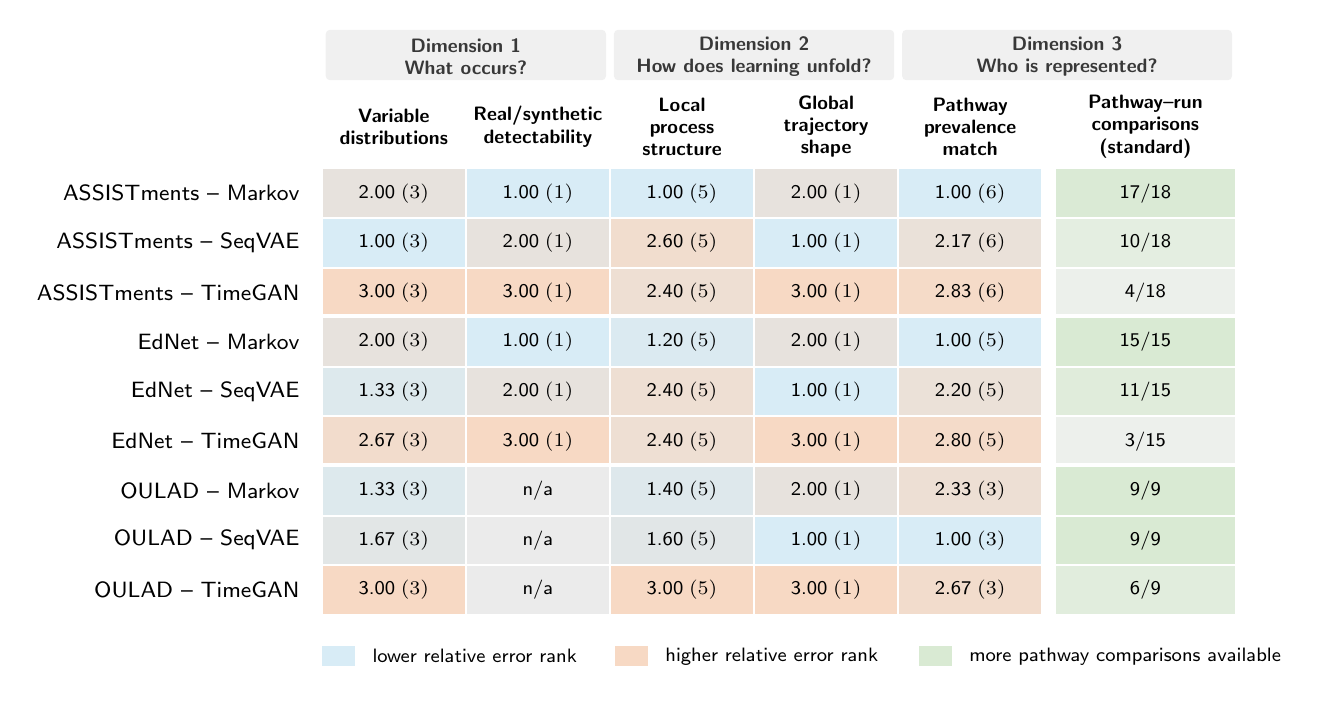
\begin{tikzpicture}[x=1cm,y=1cm,font=\sffamily]
\definecolor{rankbest}{HTML}{D8ECF6}
\definecolor{rankworst}{HTML}{F7D9C4}
\definecolor{supportbest}{HTML}{D9EAD3}
\definecolor{supportworst}{HTML}{F2F2F2}
\fill[black!6,rounded corners=1.5pt] (4.050,1.760) rectangle (7.610,1.120);
\node[align=center,font=\sffamily\bfseries\scriptsize,text=black!78] at (5.830,1.420) {Dimension 1\\What occurs?};
\fill[black!6,rounded corners=1.5pt] (7.710,1.760) rectangle (11.270,1.120);
\node[align=center,font=\sffamily\bfseries\scriptsize,text=black!78] at (9.490,1.420) {Dimension 2\\How does learning unfold?};
\fill[black!6,rounded corners=1.5pt] (11.370,1.760) rectangle (15.560,1.120);
\node[align=center,font=\sffamily\bfseries\scriptsize,text=black!78] at (13.465,1.420) {Dimension 3\\Who is represented?};
\node[align=center,font=\sffamily\bfseries\scriptsize] at (4.915,0.530) {Variable\\distributions};
\node[align=center,font=\sffamily\bfseries\scriptsize] at (6.745,0.530) {Real/synthetic\\detectability};
\node[align=center,font=\sffamily\bfseries\scriptsize] at (8.575,0.530) {Local\\process\\structure};
\node[align=center,font=\sffamily\bfseries\scriptsize] at (10.405,0.530) {Global\\trajectory\\shape};
\node[align=center,font=\sffamily\bfseries\scriptsize] at (12.235,0.530) {Pathway\\prevalence\\match};
\node[align=center,font=\sffamily\bfseries\scriptsize] at (14.460,0.530) {Pathway--run\\comparisons\\(standard)};
\node[anchor=east,font=\sffamily\footnotesize] at (3.840,-0.315) {ASSISTments -- Markov};
\fill[rankbest!50!rankworst] (4.000,0.000) rectangle (5.830,-0.630);
\draw[white,line width=0.7pt] (4.000,0.000) rectangle (5.830,-0.630);
\node[align=center,font=\sffamily\scriptsize] at (4.915,-0.315) {2.00\;\textnormal{(3)}};
\fill[rankbest!100!rankworst] (5.830,0.000) rectangle (7.660,-0.630);
\draw[white,line width=0.7pt] (5.830,0.000) rectangle (7.660,-0.630);
\node[align=center,font=\sffamily\scriptsize] at (6.745,-0.315) {1.00\;\textnormal{(1)}};
\fill[rankbest!100!rankworst] (7.660,0.000) rectangle (9.490,-0.630);
\draw[white,line width=0.7pt] (7.660,0.000) rectangle (9.490,-0.630);
\node[align=center,font=\sffamily\scriptsize] at (8.575,-0.315) {1.00\;\textnormal{(5)}};
\fill[rankbest!50!rankworst] (9.490,0.000) rectangle (11.320,-0.630);
\draw[white,line width=0.7pt] (9.490,0.000) rectangle (11.320,-0.630);
\node[align=center,font=\sffamily\scriptsize] at (10.405,-0.315) {2.00\;\textnormal{(1)}};
\fill[rankbest!100!rankworst] (11.320,0.000) rectangle (13.150,-0.630);
\draw[white,line width=0.7pt] (11.320,0.000) rectangle (13.150,-0.630);
\node[align=center,font=\sffamily\scriptsize] at (12.235,-0.315) {1.00\;\textnormal{(6)}};
\fill[supportbest!94!supportworst] (13.310,0.000) rectangle (15.610,-0.630);
\draw[white,line width=0.7pt] (13.310,0.000) rectangle (15.610,-0.630);
\node[align=center,font=\sffamily\scriptsize] at (14.460,-0.315) {17/18};
\node[anchor=east,font=\sffamily\footnotesize] at (3.840,-0.945) {ASSISTments -- SeqVAE};
\fill[rankbest!100!rankworst] (4.000,-0.630) rectangle (5.830,-1.260);
\draw[white,line width=0.7pt] (4.000,-0.630) rectangle (5.830,-1.260);
\node[align=center,font=\sffamily\scriptsize] at (4.915,-0.945) {1.00\;\textnormal{(3)}};
\fill[rankbest!50!rankworst] (5.830,-0.630) rectangle (7.660,-1.260);
\draw[white,line width=0.7pt] (5.830,-0.630) rectangle (7.660,-1.260);
\node[align=center,font=\sffamily\scriptsize] at (6.745,-0.945) {2.00\;\textnormal{(1)}};
\fill[rankbest!20!rankworst] (7.660,-0.630) rectangle (9.490,-1.260);
\draw[white,line width=0.7pt] (7.660,-0.630) rectangle (9.490,-1.260);
\node[align=center,font=\sffamily\scriptsize] at (8.575,-0.945) {2.60\;\textnormal{(5)}};
\fill[rankbest!100!rankworst] (9.490,-0.630) rectangle (11.320,-1.260);
\draw[white,line width=0.7pt] (9.490,-0.630) rectangle (11.320,-1.260);
\node[align=center,font=\sffamily\scriptsize] at (10.405,-0.945) {1.00\;\textnormal{(1)}};
\fill[rankbest!42!rankworst] (11.320,-0.630) rectangle (13.150,-1.260);
\draw[white,line width=0.7pt] (11.320,-0.630) rectangle (13.150,-1.260);
\node[align=center,font=\sffamily\scriptsize] at (12.235,-0.945) {2.17\;\textnormal{(6)}};
\fill[supportbest!56!supportworst] (13.310,-0.630) rectangle (15.610,-1.260);
\draw[white,line width=0.7pt] (13.310,-0.630) rectangle (15.610,-1.260);
\node[align=center,font=\sffamily\scriptsize] at (14.460,-0.945) {10/18};
\node[anchor=east,font=\sffamily\footnotesize] at (3.840,-1.575) {ASSISTments -- TimeGAN};
\fill[rankbest!0!rankworst] (4.000,-1.260) rectangle (5.830,-1.890);
\draw[white,line width=0.7pt] (4.000,-1.260) rectangle (5.830,-1.890);
\node[align=center,font=\sffamily\scriptsize] at (4.915,-1.575) {3.00\;\textnormal{(3)}};
\fill[rankbest!0!rankworst] (5.830,-1.260) rectangle (7.660,-1.890);
\draw[white,line width=0.7pt] (5.830,-1.260) rectangle (7.660,-1.890);
\node[align=center,font=\sffamily\scriptsize] at (6.745,-1.575) {3.00\;\textnormal{(1)}};
\fill[rankbest!30!rankworst] (7.660,-1.260) rectangle (9.490,-1.890);
\draw[white,line width=0.7pt] (7.660,-1.260) rectangle (9.490,-1.890);
\node[align=center,font=\sffamily\scriptsize] at (8.575,-1.575) {2.40\;\textnormal{(5)}};
\fill[rankbest!0!rankworst] (9.490,-1.260) rectangle (11.320,-1.890);
\draw[white,line width=0.7pt] (9.490,-1.260) rectangle (11.320,-1.890);
\node[align=center,font=\sffamily\scriptsize] at (10.405,-1.575) {3.00\;\textnormal{(1)}};
\fill[rankbest!8!rankworst] (11.320,-1.260) rectangle (13.150,-1.890);
\draw[white,line width=0.7pt] (11.320,-1.260) rectangle (13.150,-1.890);
\node[align=center,font=\sffamily\scriptsize] at (12.235,-1.575) {2.83\;\textnormal{(6)}};
\fill[supportbest!22!supportworst] (13.310,-1.260) rectangle (15.610,-1.890);
\draw[white,line width=0.7pt] (13.310,-1.260) rectangle (15.610,-1.890);
\node[align=center,font=\sffamily\scriptsize] at (14.460,-1.575) {4/18};
\draw[white,line width=2.2pt] (4.000,-1.890) -- (15.610,-1.890);
\node[anchor=east,font=\sffamily\footnotesize] at (3.840,-2.205) {EdNet -- Markov};
\fill[rankbest!50!rankworst] (4.000,-1.890) rectangle (5.830,-2.520);
\draw[white,line width=0.7pt] (4.000,-1.890) rectangle (5.830,-2.520);
\node[align=center,font=\sffamily\scriptsize] at (4.915,-2.205) {2.00\;\textnormal{(3)}};
\fill[rankbest!100!rankworst] (5.830,-1.890) rectangle (7.660,-2.520);
\draw[white,line width=0.7pt] (5.830,-1.890) rectangle (7.660,-2.520);
\node[align=center,font=\sffamily\scriptsize] at (6.745,-2.205) {1.00\;\textnormal{(1)}};
\fill[rankbest!90!rankworst] (7.660,-1.890) rectangle (9.490,-2.520);
\draw[white,line width=0.7pt] (7.660,-1.890) rectangle (9.490,-2.520);
\node[align=center,font=\sffamily\scriptsize] at (8.575,-2.205) {1.20\;\textnormal{(5)}};
\fill[rankbest!50!rankworst] (9.490,-1.890) rectangle (11.320,-2.520);
\draw[white,line width=0.7pt] (9.490,-1.890) rectangle (11.320,-2.520);
\node[align=center,font=\sffamily\scriptsize] at (10.405,-2.205) {2.00\;\textnormal{(1)}};
\fill[rankbest!100!rankworst] (11.320,-1.890) rectangle (13.150,-2.520);
\draw[white,line width=0.7pt] (11.320,-1.890) rectangle (13.150,-2.520);
\node[align=center,font=\sffamily\scriptsize] at (12.235,-2.205) {1.00\;\textnormal{(5)}};
\fill[supportbest!100!supportworst] (13.310,-1.890) rectangle (15.610,-2.520);
\draw[white,line width=0.7pt] (13.310,-1.890) rectangle (15.610,-2.520);
\node[align=center,font=\sffamily\scriptsize] at (14.460,-2.205) {15/15};
\node[anchor=east,font=\sffamily\footnotesize] at (3.840,-2.835) {EdNet -- SeqVAE};
\fill[rankbest!83!rankworst] (4.000,-2.520) rectangle (5.830,-3.150);
\draw[white,line width=0.7pt] (4.000,-2.520) rectangle (5.830,-3.150);
\node[align=center,font=\sffamily\scriptsize] at (4.915,-2.835) {1.33\;\textnormal{(3)}};
\fill[rankbest!50!rankworst] (5.830,-2.520) rectangle (7.660,-3.150);
\draw[white,line width=0.7pt] (5.830,-2.520) rectangle (7.660,-3.150);
\node[align=center,font=\sffamily\scriptsize] at (6.745,-2.835) {2.00\;\textnormal{(1)}};
\fill[rankbest!30!rankworst] (7.660,-2.520) rectangle (9.490,-3.150);
\draw[white,line width=0.7pt] (7.660,-2.520) rectangle (9.490,-3.150);
\node[align=center,font=\sffamily\scriptsize] at (8.575,-2.835) {2.40\;\textnormal{(5)}};
\fill[rankbest!100!rankworst] (9.490,-2.520) rectangle (11.320,-3.150);
\draw[white,line width=0.7pt] (9.490,-2.520) rectangle (11.320,-3.150);
\node[align=center,font=\sffamily\scriptsize] at (10.405,-2.835) {1.00\;\textnormal{(1)}};
\fill[rankbest!40!rankworst] (11.320,-2.520) rectangle (13.150,-3.150);
\draw[white,line width=0.7pt] (11.320,-2.520) rectangle (13.150,-3.150);
\node[align=center,font=\sffamily\scriptsize] at (12.235,-2.835) {2.20\;\textnormal{(5)}};
\fill[supportbest!73!supportworst] (13.310,-2.520) rectangle (15.610,-3.150);
\draw[white,line width=0.7pt] (13.310,-2.520) rectangle (15.610,-3.150);
\node[align=center,font=\sffamily\scriptsize] at (14.460,-2.835) {11/15};
\node[anchor=east,font=\sffamily\footnotesize] at (3.840,-3.465) {EdNet -- TimeGAN};
\fill[rankbest!17!rankworst] (4.000,-3.150) rectangle (5.830,-3.780);
\draw[white,line width=0.7pt] (4.000,-3.150) rectangle (5.830,-3.780);
\node[align=center,font=\sffamily\scriptsize] at (4.915,-3.465) {2.67\;\textnormal{(3)}};
\fill[rankbest!0!rankworst] (5.830,-3.150) rectangle (7.660,-3.780);
\draw[white,line width=0.7pt] (5.830,-3.150) rectangle (7.660,-3.780);
\node[align=center,font=\sffamily\scriptsize] at (6.745,-3.465) {3.00\;\textnormal{(1)}};
\fill[rankbest!30!rankworst] (7.660,-3.150) rectangle (9.490,-3.780);
\draw[white,line width=0.7pt] (7.660,-3.150) rectangle (9.490,-3.780);
\node[align=center,font=\sffamily\scriptsize] at (8.575,-3.465) {2.40\;\textnormal{(5)}};
\fill[rankbest!0!rankworst] (9.490,-3.150) rectangle (11.320,-3.780);
\draw[white,line width=0.7pt] (9.490,-3.150) rectangle (11.320,-3.780);
\node[align=center,font=\sffamily\scriptsize] at (10.405,-3.465) {3.00\;\textnormal{(1)}};
\fill[rankbest!10!rankworst] (11.320,-3.150) rectangle (13.150,-3.780);
\draw[white,line width=0.7pt] (11.320,-3.150) rectangle (13.150,-3.780);
\node[align=center,font=\sffamily\scriptsize] at (12.235,-3.465) {2.80\;\textnormal{(5)}};
\fill[supportbest!20!supportworst] (13.310,-3.150) rectangle (15.610,-3.780);
\draw[white,line width=0.7pt] (13.310,-3.150) rectangle (15.610,-3.780);
\node[align=center,font=\sffamily\scriptsize] at (14.460,-3.465) {3/15};
\draw[white,line width=2.2pt] (4.000,-3.780) -- (15.610,-3.780);
\node[anchor=east,font=\sffamily\footnotesize] at (3.840,-4.095) {OULAD -- Markov};
\fill[rankbest!83!rankworst] (4.000,-3.780) rectangle (5.830,-4.410);
\draw[white,line width=0.7pt] (4.000,-3.780) rectangle (5.830,-4.410);
\node[align=center,font=\sffamily\scriptsize] at (4.915,-4.095) {1.33\;\textnormal{(3)}};
\fill[gray!16] (5.830,-3.780) rectangle (7.660,-4.410);
\draw[white,line width=0.7pt] (5.830,-3.780) rectangle (7.660,-4.410);
\node[align=center,font=\sffamily\scriptsize] at (6.745,-4.095) {n/a};
\fill[rankbest!80!rankworst] (7.660,-3.780) rectangle (9.490,-4.410);
\draw[white,line width=0.7pt] (7.660,-3.780) rectangle (9.490,-4.410);
\node[align=center,font=\sffamily\scriptsize] at (8.575,-4.095) {1.40\;\textnormal{(5)}};
\fill[rankbest!50!rankworst] (9.490,-3.780) rectangle (11.320,-4.410);
\draw[white,line width=0.7pt] (9.490,-3.780) rectangle (11.320,-4.410);
\node[align=center,font=\sffamily\scriptsize] at (10.405,-4.095) {2.00\;\textnormal{(1)}};
\fill[rankbest!33!rankworst] (11.320,-3.780) rectangle (13.150,-4.410);
\draw[white,line width=0.7pt] (11.320,-3.780) rectangle (13.150,-4.410);
\node[align=center,font=\sffamily\scriptsize] at (12.235,-4.095) {2.33\;\textnormal{(3)}};
\fill[supportbest!100!supportworst] (13.310,-3.780) rectangle (15.610,-4.410);
\draw[white,line width=0.7pt] (13.310,-3.780) rectangle (15.610,-4.410);
\node[align=center,font=\sffamily\scriptsize] at (14.460,-4.095) {9/9};
\node[anchor=east,font=\sffamily\footnotesize] at (3.840,-4.725) {OULAD -- SeqVAE};
\fill[rankbest!67!rankworst] (4.000,-4.410) rectangle (5.830,-5.040);
\draw[white,line width=0.7pt] (4.000,-4.410) rectangle (5.830,-5.040);
\node[align=center,font=\sffamily\scriptsize] at (4.915,-4.725) {1.67\;\textnormal{(3)}};
\fill[gray!16] (5.830,-4.410) rectangle (7.660,-5.040);
\draw[white,line width=0.7pt] (5.830,-4.410) rectangle (7.660,-5.040);
\node[align=center,font=\sffamily\scriptsize] at (6.745,-4.725) {n/a};
\fill[rankbest!70!rankworst] (7.660,-4.410) rectangle (9.490,-5.040);
\draw[white,line width=0.7pt] (7.660,-4.410) rectangle (9.490,-5.040);
\node[align=center,font=\sffamily\scriptsize] at (8.575,-4.725) {1.60\;\textnormal{(5)}};
\fill[rankbest!100!rankworst] (9.490,-4.410) rectangle (11.320,-5.040);
\draw[white,line width=0.7pt] (9.490,-4.410) rectangle (11.320,-5.040);
\node[align=center,font=\sffamily\scriptsize] at (10.405,-4.725) {1.00\;\textnormal{(1)}};
\fill[rankbest!100!rankworst] (11.320,-4.410) rectangle (13.150,-5.040);
\draw[white,line width=0.7pt] (11.320,-4.410) rectangle (13.150,-5.040);
\node[align=center,font=\sffamily\scriptsize] at (12.235,-4.725) {1.00\;\textnormal{(3)}};
\fill[supportbest!100!supportworst] (13.310,-4.410) rectangle (15.610,-5.040);
\draw[white,line width=0.7pt] (13.310,-4.410) rectangle (15.610,-5.040);
\node[align=center,font=\sffamily\scriptsize] at (14.460,-4.725) {9/9};
\node[anchor=east,font=\sffamily\footnotesize] at (3.840,-5.355) {OULAD -- TimeGAN};
\fill[rankbest!0!rankworst] (4.000,-5.040) rectangle (5.830,-5.670);
\draw[white,line width=0.7pt] (4.000,-5.040) rectangle (5.830,-5.670);
\node[align=center,font=\sffamily\scriptsize] at (4.915,-5.355) {3.00\;\textnormal{(3)}};
\fill[gray!16] (5.830,-5.040) rectangle (7.660,-5.670);
\draw[white,line width=0.7pt] (5.830,-5.040) rectangle (7.660,-5.670);
\node[align=center,font=\sffamily\scriptsize] at (6.745,-5.355) {n/a};
\fill[rankbest!0!rankworst] (7.660,-5.040) rectangle (9.490,-5.670);
\draw[white,line width=0.7pt] (7.660,-5.040) rectangle (9.490,-5.670);
\node[align=center,font=\sffamily\scriptsize] at (8.575,-5.355) {3.00\;\textnormal{(5)}};
\fill[rankbest!0!rankworst] (9.490,-5.040) rectangle (11.320,-5.670);
\draw[white,line width=0.7pt] (9.490,-5.040) rectangle (11.320,-5.670);
\node[align=center,font=\sffamily\scriptsize] at (10.405,-5.355) {3.00\;\textnormal{(1)}};
\fill[rankbest!17!rankworst] (11.320,-5.040) rectangle (13.150,-5.670);
\draw[white,line width=0.7pt] (11.320,-5.040) rectangle (13.150,-5.670);
\node[align=center,font=\sffamily\scriptsize] at (12.235,-5.355) {2.67\;\textnormal{(3)}};
\fill[supportbest!67!supportworst] (13.310,-5.040) rectangle (15.610,-5.670);
\draw[white,line width=0.7pt] (13.310,-5.040) rectangle (15.610,-5.670);
\node[align=center,font=\sffamily\scriptsize] at (14.460,-5.355) {6/9};
\fill[rankbest] (4.000,-6.070) rectangle (4.420,-6.320);
\node[anchor=west,font=\sffamily\scriptsize] at (4.520,-6.195) {lower relative error rank};
\fill[rankworst] (7.720,-6.070) rectangle (8.140,-6.320);
\node[anchor=west,font=\sffamily\scriptsize] at (8.240,-6.195) {higher relative error rank};
\fill[supportbest] (11.580,-6.070) rectangle (12.000,-6.320);
\node[anchor=west,font=\sffamily\scriptsize] at (12.100,-6.195) {more pathway comparisons available};
\end{tikzpicture}
}
\caption{RQ1 preservation profile. Cells average relative error ranks over metrics calculable for all generators and seeds (metric counts in parentheses); lower is closer to real training data. OULAD full-record detectability is not generator-comparable (n/a). Available pathway--run comparisons count standard-generation pathway--seed combinations with at least ten qualifying real and ten qualifying synthetic learners, out of all eligible combinations.}
\label{fig:rq1-construct-profile}
\end{figure}

\paragraph{Responses and activities across learners.}
SeqVAE most closely reproduced visible composition in the tutoring datasets, whereas Markov was closest for OULAD. Yet matching individual variables did not ensure realistic records: ASSISTments SeqVAE behavior-rate error was only \(0.12\pm0.08\) percentage points, while source-detection AUROC was \(0.8500\pm0.0008\), compared with Markov's near-chance \(0.5334\pm0.0037\). OULAD full-record detectability remains excluded because of shared profile and outcome construction.

\paragraph{Learning over time.}
Markov had the lowest aggregated local-process error rank in all datasets, although individual metrics varied. ASSISTments three-event sequence divergence was \(0.0828\pm0.0006\) for Markov versus \(0.8635\pm0.0032\) for SeqVAE. Conversely, SeqVAE most closely retained global early-to-late shape in every dataset, the EdNet response-gap signal, and the OULAD inactivity-gap signal. Local order and overall development therefore favored different generators.

\paragraph{Uncommon pathways.}
Pathway-prevalence errors included no qualifying synthetic trajectories and severe overproduction; Section~\ref{sec:window-assembly} relates the largest errors to window assembly. The rare-skill pathway occurred among 4.87\% of real ASSISTments learners but \(98.52\pm0.73\)\% of SeqVAE learners. TimeGAN also often produced too few qualifying learners for within-pathway behavioral comparisons (Figure~\ref{fig:rq1-construct-profile}). The supplement retains signed prevalence for all 42 comparisons and support counts for every included or omitted pathway--seed comparison.

\subsection{RQ2: Prediction Within Pathways and Effects of Targeting}
\label{sec:rq2-results}

\textbf{Answer to RQ2.} Standard synthetic-only training reduced mean overall prediction performance in every dataset--generator combination, but within-pathway results included both losses and gains. Targeting did not consistently improve pathway representation and predictive usefulness together.

\paragraph{Overall prediction.}
Figure~\ref{fig:rq2-utility-targeting} shows overall primary-task performance. Every standard synthetic-only predictor had lower mean AUPRC than its real-only counterpart. Markov had the smallest loss on ASSISTments (\(0.0276\pm0.0002\)), EdNet (\(0.0308\pm0.0012\)), and OULAD (\(0.0234\pm0.0006\)); the other generators lost more utility in every dataset. Neither standard nor targeted augmentation had a positive mean change over real-only AUPRC in any of the nine dataset--generator combinations (Supplementary Table~S12). Thus, adding either type of synthetic data did not improve mean next-step prediction on real learners.

\begin{figure}[!htbp]
\centering
\resizebox{\linewidth}{!}{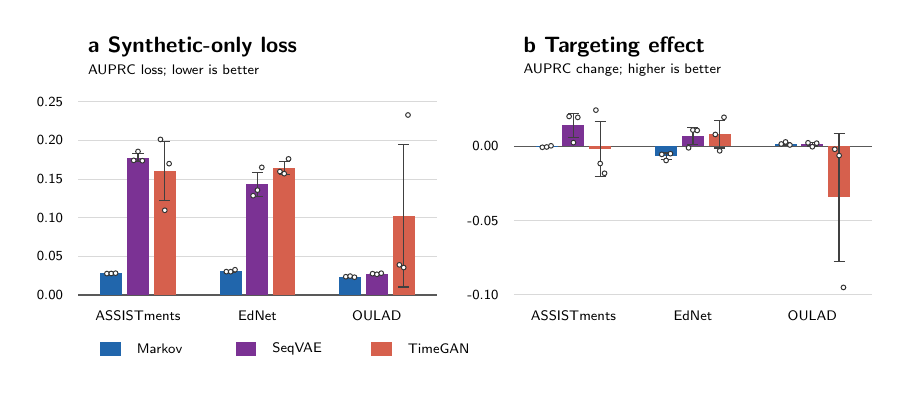
\begin{tikzpicture}[x=1cm,y=1cm,font=\sffamily]
\definecolor{paperblue}{HTML}{2166AC}
\definecolor{paperpurple}{HTML}{7B3294}
\definecolor{paperred}{HTML}{D6604D}
\definecolor{papergreen}{HTML}{4D9221}
\definecolor{paperpink}{HTML}{C51B7D}
\node[anchor=west,font=\sffamily\bfseries\footnotesize] at (1.020,3.600) {a  Synthetic-only loss};
\node[anchor=west,font=\sffamily\tiny] at (1.020,3.300) {AUPRC loss; lower is better};
\draw[gray!30,line width=0.35pt] (1.020,0.450) -- (5.570,0.450);
\node[anchor=east,font=\sffamily\tiny] at (0.950,0.450) {0.00};
\draw[gray!30,line width=0.35pt] (1.020,0.940) -- (5.570,0.940);
\node[anchor=east,font=\sffamily\tiny] at (0.950,0.940) {0.05};
\draw[gray!30,line width=0.35pt] (1.020,1.430) -- (5.570,1.430);
\node[anchor=east,font=\sffamily\tiny] at (0.950,1.430) {0.10};
\draw[gray!30,line width=0.35pt] (1.020,1.920) -- (5.570,1.920);
\node[anchor=east,font=\sffamily\tiny] at (0.950,1.920) {0.15};
\draw[gray!30,line width=0.35pt] (1.020,2.410) -- (5.570,2.410);
\node[anchor=east,font=\sffamily\tiny] at (0.950,2.410) {0.20};
\draw[gray!30,line width=0.35pt] (1.020,2.900) -- (5.570,2.900);
\node[anchor=east,font=\sffamily\tiny] at (0.950,2.900) {0.25};
\draw[black!65,line width=0.55pt] (1.020,0.450) -- (5.570,0.450);
\node[align=center,font=\sffamily\tiny] at (1.778,0.180) {ASSISTments};
\fill[paperblue] (1.298,0.450) rectangle (1.578,0.721);
\draw[black!75,line width=0.45pt] (1.438,0.719) -- (1.438,0.723);
\draw[black!75,line width=0.45pt] (1.368,0.719) -- (1.508,0.719);
\draw[black!75,line width=0.45pt] (1.368,0.723) -- (1.508,0.723);
\fill[white] (1.383,0.719) circle (0.030);
\draw[black!80,line width=0.35pt] (1.383,0.719) circle (0.030);
\fill[white] (1.438,0.720) circle (0.030);
\draw[black!80,line width=0.35pt] (1.438,0.720) circle (0.030);
\fill[white] (1.493,0.724) circle (0.030);
\draw[black!80,line width=0.35pt] (1.493,0.724) circle (0.030);
\fill[paperpurple] (1.638,0.450) rectangle (1.918,2.193);
\draw[black!75,line width=0.45pt] (1.778,2.139) -- (1.778,2.248);
\draw[black!75,line width=0.45pt] (1.708,2.139) -- (1.848,2.139);
\draw[black!75,line width=0.45pt] (1.708,2.248) -- (1.848,2.248);
\fill[white] (1.723,2.157) circle (0.030);
\draw[black!80,line width=0.35pt] (1.723,2.157) circle (0.030);
\fill[white] (1.778,2.270) circle (0.030);
\draw[black!80,line width=0.35pt] (1.778,2.270) circle (0.030);
\fill[white] (1.833,2.152) circle (0.030);
\draw[black!80,line width=0.35pt] (1.833,2.152) circle (0.030);
\fill[paperred] (1.978,0.450) rectangle (2.258,2.020);
\draw[black!75,line width=0.45pt] (2.118,1.647) -- (2.118,2.394);
\draw[black!75,line width=0.45pt] (2.048,1.647) -- (2.188,1.647);
\draw[black!75,line width=0.45pt] (2.048,2.394) -- (2.188,2.394);
\fill[white] (2.063,2.423) circle (0.030);
\draw[black!80,line width=0.35pt] (2.063,2.423) circle (0.030);
\fill[white] (2.118,1.523) circle (0.030);
\draw[black!80,line width=0.35pt] (2.118,1.523) circle (0.030);
\fill[white] (2.173,2.115) circle (0.030);
\draw[black!80,line width=0.35pt] (2.173,2.115) circle (0.030);
\node[align=center,font=\sffamily\tiny] at (3.295,0.180) {EdNet};
\fill[paperblue] (2.815,0.450) rectangle (3.095,0.752);
\draw[black!75,line width=0.45pt] (2.955,0.740) -- (2.955,0.763);
\draw[black!75,line width=0.45pt] (2.885,0.740) -- (3.025,0.740);
\draw[black!75,line width=0.45pt] (2.885,0.763) -- (3.025,0.763);
\fill[white] (2.900,0.744) circle (0.030);
\draw[black!80,line width=0.35pt] (2.900,0.744) circle (0.030);
\fill[white] (2.955,0.743) circle (0.030);
\draw[black!80,line width=0.35pt] (2.955,0.743) circle (0.030);
\fill[white] (3.010,0.768) circle (0.030);
\draw[black!80,line width=0.35pt] (3.010,0.768) circle (0.030);
\fill[paperpurple] (3.155,0.450) rectangle (3.435,1.851);
\draw[black!75,line width=0.45pt] (3.295,1.696) -- (3.295,2.007);
\draw[black!75,line width=0.45pt] (3.225,1.696) -- (3.365,1.696);
\draw[black!75,line width=0.45pt] (3.225,2.007) -- (3.365,2.007);
\fill[white] (3.240,1.708) circle (0.030);
\draw[black!80,line width=0.35pt] (3.240,1.708) circle (0.030);
\fill[white] (3.295,1.779) circle (0.030);
\draw[black!80,line width=0.35pt] (3.295,1.779) circle (0.030);
\fill[white] (3.350,2.068) circle (0.030);
\draw[black!80,line width=0.35pt] (3.350,2.068) circle (0.030);
\fill[paperred] (3.495,0.450) rectangle (3.775,2.060);
\draw[black!75,line width=0.45pt] (3.635,1.977) -- (3.635,2.142);
\draw[black!75,line width=0.45pt] (3.565,1.977) -- (3.705,1.977);
\draw[black!75,line width=0.45pt] (3.565,2.142) -- (3.705,2.142);
\fill[white] (3.580,2.015) circle (0.030);
\draw[black!80,line width=0.35pt] (3.580,2.015) circle (0.030);
\fill[white] (3.635,1.988) circle (0.030);
\draw[black!80,line width=0.35pt] (3.635,1.988) circle (0.030);
\fill[white] (3.690,2.176) circle (0.030);
\draw[black!80,line width=0.35pt] (3.690,2.176) circle (0.030);
\node[align=center,font=\sffamily\tiny] at (4.812,0.180) {OULAD};
\fill[paperblue] (4.332,0.450) rectangle (4.612,0.679);
\draw[black!75,line width=0.45pt] (4.472,0.674) -- (4.472,0.685);
\draw[black!75,line width=0.45pt] (4.402,0.674) -- (4.542,0.674);
\draw[black!75,line width=0.45pt] (4.402,0.685) -- (4.542,0.685);
\fill[white] (4.417,0.679) circle (0.030);
\draw[black!80,line width=0.35pt] (4.417,0.679) circle (0.030);
\fill[white] (4.472,0.687) circle (0.030);
\draw[black!80,line width=0.35pt] (4.472,0.687) circle (0.030);
\fill[white] (4.527,0.673) circle (0.030);
\draw[black!80,line width=0.35pt] (4.527,0.673) circle (0.030);
\fill[paperpurple] (4.672,0.450) rectangle (4.952,0.718);
\draw[black!75,line width=0.45pt] (4.812,0.712) -- (4.812,0.723);
\draw[black!75,line width=0.45pt] (4.742,0.712) -- (4.882,0.712);
\draw[black!75,line width=0.45pt] (4.742,0.723) -- (4.882,0.723);
\fill[white] (4.757,0.718) circle (0.030);
\draw[black!80,line width=0.35pt] (4.757,0.718) circle (0.030);
\fill[white] (4.812,0.710) circle (0.030);
\draw[black!80,line width=0.35pt] (4.812,0.710) circle (0.030);
\fill[white] (4.867,0.724) circle (0.030);
\draw[black!80,line width=0.35pt] (4.867,0.724) circle (0.030);
\fill[paperred] (5.012,0.450) rectangle (5.292,1.453);
\draw[black!75,line width=0.45pt] (5.152,0.548) -- (5.152,2.358);
\draw[black!75,line width=0.45pt] (5.082,0.548) -- (5.222,0.548);
\draw[black!75,line width=0.45pt] (5.082,2.358) -- (5.222,2.358);
\fill[white] (5.097,0.830) circle (0.030);
\draw[black!80,line width=0.35pt] (5.097,0.830) circle (0.030);
\fill[white] (5.152,0.796) circle (0.030);
\draw[black!80,line width=0.35pt] (5.152,0.796) circle (0.030);
\fill[white] (5.207,2.733) circle (0.030);
\draw[black!80,line width=0.35pt] (5.207,2.733) circle (0.030);
\node[anchor=west,font=\sffamily\bfseries\footnotesize] at (6.550,3.600) {b  Targeting effect};
\node[anchor=west,font=\sffamily\tiny] at (6.550,3.300) {AUPRC change; higher is better};
\draw[gray!30,line width=0.35pt] (6.550,0.450) -- (11.100,0.450);
\node[anchor=east,font=\sffamily\tiny] at (6.480,0.450) {-0.10};
\draw[gray!30,line width=0.35pt] (6.550,1.392) -- (11.100,1.392);
\node[anchor=east,font=\sffamily\tiny] at (6.480,1.392) {-0.05};
\draw[gray!30,line width=0.35pt] (6.550,2.335) -- (11.100,2.335);
\node[anchor=east,font=\sffamily\tiny] at (6.480,2.335) {0.00};
\draw[black!65,line width=0.55pt] (6.550,2.335) -- (11.100,2.335);
\node[align=center,font=\sffamily\tiny] at (7.308,0.180) {ASSISTments};
\fill[paperblue] (6.828,2.331) rectangle (7.108,2.335);
\draw[black!75,line width=0.45pt] (6.968,2.323) -- (6.968,2.339);
\draw[black!75,line width=0.45pt] (6.898,2.323) -- (7.038,2.323);
\draw[black!75,line width=0.45pt] (6.898,2.339) -- (7.038,2.339);
\fill[white] (6.913,2.323) circle (0.030);
\draw[black!80,line width=0.35pt] (6.913,2.323) circle (0.030);
\fill[white] (6.968,2.327) circle (0.030);
\draw[black!80,line width=0.35pt] (6.968,2.327) circle (0.030);
\fill[white] (7.023,2.342) circle (0.030);
\draw[black!80,line width=0.35pt] (7.023,2.342) circle (0.030);
\fill[paperpurple] (7.168,2.335) rectangle (7.448,2.600);
\draw[black!75,line width=0.45pt] (7.308,2.447) -- (7.308,2.754);
\draw[black!75,line width=0.45pt] (7.238,2.447) -- (7.378,2.447);
\draw[black!75,line width=0.45pt] (7.238,2.754) -- (7.378,2.754);
\fill[white] (7.253,2.715) circle (0.030);
\draw[black!80,line width=0.35pt] (7.253,2.715) circle (0.030);
\fill[white] (7.308,2.383) circle (0.030);
\draw[black!80,line width=0.35pt] (7.308,2.383) circle (0.030);
\fill[white] (7.363,2.703) circle (0.030);
\draw[black!80,line width=0.35pt] (7.363,2.703) circle (0.030);
\fill[paperred] (7.508,2.302) rectangle (7.788,2.335);
\draw[black!75,line width=0.45pt] (7.648,1.949) -- (7.648,2.655);
\draw[black!75,line width=0.45pt] (7.578,1.949) -- (7.718,1.949);
\draw[black!75,line width=0.45pt] (7.578,2.655) -- (7.718,2.655);
\fill[white] (7.593,2.795) circle (0.030);
\draw[black!80,line width=0.35pt] (7.593,2.795) circle (0.030);
\fill[white] (7.648,2.117) circle (0.030);
\draw[black!80,line width=0.35pt] (7.648,2.117) circle (0.030);
\fill[white] (7.703,1.993) circle (0.030);
\draw[black!80,line width=0.35pt] (7.703,1.993) circle (0.030);
\node[align=center,font=\sffamily\tiny] at (8.825,0.180) {EdNet};
\fill[paperblue] (8.345,2.210) rectangle (8.625,2.335);
\draw[black!75,line width=0.45pt] (8.485,2.172) -- (8.485,2.249);
\draw[black!75,line width=0.45pt] (8.415,2.172) -- (8.555,2.172);
\draw[black!75,line width=0.45pt] (8.415,2.249) -- (8.555,2.249);
\fill[white] (8.430,2.233) circle (0.030);
\draw[black!80,line width=0.35pt] (8.430,2.233) circle (0.030);
\fill[white] (8.485,2.156) circle (0.030);
\draw[black!80,line width=0.35pt] (8.485,2.156) circle (0.030);
\fill[white] (8.540,2.242) circle (0.030);
\draw[black!80,line width=0.35pt] (8.540,2.242) circle (0.030);
\fill[paperpurple] (8.685,2.335) rectangle (8.965,2.465);
\draw[black!75,line width=0.45pt] (8.825,2.359) -- (8.825,2.570);
\draw[black!75,line width=0.45pt] (8.755,2.359) -- (8.895,2.359);
\draw[black!75,line width=0.45pt] (8.755,2.570) -- (8.895,2.570);
\fill[white] (8.770,2.316) circle (0.030);
\draw[black!80,line width=0.35pt] (8.770,2.316) circle (0.030);
\fill[white] (8.825,2.542) circle (0.030);
\draw[black!80,line width=0.35pt] (8.825,2.542) circle (0.030);
\fill[white] (8.880,2.537) circle (0.030);
\draw[black!80,line width=0.35pt] (8.880,2.537) circle (0.030);
\fill[paperred] (9.025,2.335) rectangle (9.305,2.489);
\draw[black!75,line width=0.45pt] (9.165,2.315) -- (9.165,2.663);
\draw[black!75,line width=0.45pt] (9.095,2.315) -- (9.235,2.315);
\draw[black!75,line width=0.45pt] (9.095,2.663) -- (9.235,2.663);
\fill[white] (9.110,2.486) circle (0.030);
\draw[black!80,line width=0.35pt] (9.110,2.486) circle (0.030);
\fill[white] (9.165,2.278) circle (0.030);
\draw[black!80,line width=0.35pt] (9.165,2.278) circle (0.030);
\fill[white] (9.220,2.704) circle (0.030);
\draw[black!80,line width=0.35pt] (9.220,2.704) circle (0.030);
\node[align=center,font=\sffamily\tiny] at (10.342,0.180) {OULAD};
\fill[paperblue] (9.862,2.335) rectangle (10.142,2.369);
\draw[black!75,line width=0.45pt] (10.002,2.353) -- (10.002,2.386);
\draw[black!75,line width=0.45pt] (9.932,2.353) -- (10.072,2.353);
\draw[black!75,line width=0.45pt] (9.932,2.386) -- (10.072,2.386);
\fill[white] (9.947,2.365) circle (0.030);
\draw[black!80,line width=0.35pt] (9.947,2.365) circle (0.030);
\fill[white] (10.002,2.391) circle (0.030);
\draw[black!80,line width=0.35pt] (10.002,2.391) circle (0.030);
\fill[white] (10.057,2.352) circle (0.030);
\draw[black!80,line width=0.35pt] (10.057,2.352) circle (0.030);
\fill[paperpurple] (10.202,2.335) rectangle (10.482,2.362);
\draw[black!75,line width=0.45pt] (10.342,2.339) -- (10.342,2.384);
\draw[black!75,line width=0.45pt] (10.272,2.339) -- (10.412,2.339);
\draw[black!75,line width=0.45pt] (10.272,2.384) -- (10.412,2.384);
\fill[white] (10.287,2.380) circle (0.030);
\draw[black!80,line width=0.35pt] (10.287,2.380) circle (0.030);
\fill[white] (10.342,2.330) circle (0.030);
\draw[black!80,line width=0.35pt] (10.342,2.330) circle (0.030);
\fill[white] (10.397,2.375) circle (0.030);
\draw[black!80,line width=0.35pt] (10.397,2.375) circle (0.030);
\fill[paperred] (10.542,1.686) rectangle (10.822,2.335);
\draw[black!75,line width=0.45pt] (10.682,0.877) -- (10.682,2.495);
\draw[black!75,line width=0.45pt] (10.612,0.877) -- (10.752,0.877);
\draw[black!75,line width=0.45pt] (10.612,2.495) -- (10.752,2.495);
\fill[white] (10.627,2.298) circle (0.030);
\draw[black!80,line width=0.35pt] (10.627,2.298) circle (0.030);
\fill[white] (10.682,2.218) circle (0.030);
\draw[black!80,line width=0.35pt] (10.682,2.218) circle (0.030);
\fill[white] (10.737,0.543) circle (0.030);
\draw[black!80,line width=0.35pt] (10.737,0.543) circle (0.030);
\fill[paperblue] (1.300,-0.330) rectangle (1.560,-0.150);
\node[anchor=west,font=\sffamily\tiny] at (1.640,-0.240) {Markov};
\fill[paperpurple] (3.020,-0.330) rectangle (3.280,-0.150);
\node[anchor=west,font=\sffamily\tiny] at (3.360,-0.240) {SeqVAE};
\fill[paperred] (4.740,-0.330) rectangle (5.000,-0.150);
\node[anchor=west,font=\sffamily\tiny] at (5.080,-0.240) {TimeGAN};
\end{tikzpicture}
}
\caption{Overall primary-task prediction on held-out real learners. (a) Loss from training the primary predictor on standard synthetic rather than real data. (b) Targeted-minus-standard synthetic-only change. Bars show means, whiskers show population SD, and white points show the three fixed generator seeds. These are descriptive cross-seed summaries. Augmentation results are reported in Supplementary Table~S12, not in these panels.}
\label{fig:rq2-utility-targeting}
\end{figure}

\paragraph{Prediction within uncommon pathways.}
Table~\ref{tab:within-pathway-gaps} shows the baseline within-pathway prediction gap: real-only minus standard synthetic-only AUPRC for the same real test learners in each pathway group. Positive gaps indicate lower synthetic-trained performance; negative gaps indicate higher synthetic-trained performance. These differences are descriptive under one fixed split and three generator seeds.

% Source: supplement-generated/complete-publication-results.csv, rq2.tail_learnability.*.synthetic_utility_gap.auprc
\begin{table}[!htbp]
\centering
\caption{Baseline within-pathway prediction gaps: real-only minus standard synthetic-only AUPRC for the same held-out real learners in each pathway group. Positive values mean lower synthetic-trained performance; negative values mean higher synthetic-trained performance. Entries are mean $\pm$ population SD over three runs; these are descriptive differences, not significance tests.}
\label{tab:within-pathway-gaps}
\small
\setlength{\tabcolsep}{4pt}
\begin{tabular}{@{}llrrr@{}}
\toprule
Dataset & Pathway & Markov & SeqVAE & TimeGAN \\
\midrule
ASSISTments & High hint use & $+0.0847\pm0.0169$ & $+0.3313\pm0.0087$ & $+0.2850\pm0.0671$ \\
 & Late correctness decline & $-0.0008\pm0.0032$ & $+0.1860\pm0.0143$ & $+0.1898\pm0.0491$ \\
 & Persistent low correctness & $+0.0621\pm0.0070$ & $+0.1076\pm0.0071$ & $+0.0603\pm0.0670$ \\
 & Rapid low-accuracy responding & $+0.1244\pm0.0181$ & $+0.2539\pm0.0060$ & $+0.2112\pm0.0627$ \\
 & Rare skill path & $+0.0224\pm0.0078$ & $+0.1143\pm0.0348$ & $+0.0907\pm0.0480$ \\
 & Recovery & $-0.0089\pm0.0096$ & $+0.1559\pm0.0867$ & $+0.1532\pm0.0318$ \\
\addlinespace
EdNet & Late correctness decline & $+0.0140\pm0.0103$ & $+0.2451\pm0.0139$ & $+0.1602\pm0.0294$ \\
 & Persistent low correctness & $+0.0123\pm0.0023$ & $+0.0141\pm0.0021$ & $+0.0084\pm0.0134$ \\
 & Rapid low-accuracy responding & $+0.0137\pm0.0035$ & $+0.0130\pm0.0156$ & $+0.0269\pm0.0059$ \\
 & Rare skill path & $-0.0027\pm0.0030$ & $+0.0360\pm0.0154$ & $+0.0643\pm0.0178$ \\
 & Recovery & $-0.0005\pm0.0043$ & $+0.1297\pm0.0102$ & $+0.1974\pm0.0159$ \\
\addlinespace
OULAD & Late disengagement & $+0.0307\pm0.0008$ & $+0.0256\pm0.0017$ & $+0.1046\pm0.1029$ \\
 & Rare activity path & $+0.0213\pm0.0014$ & $+0.0165\pm0.0004$ & $+0.0393\pm0.0222$ \\
 & Reengagement & $-0.0443\pm0.0034$ & $+0.0096\pm0.0025$ & $+0.0597\pm0.1331$ \\
\bottomrule
\end{tabular}
\end{table}


For persistent low correctness in ASSISTments, the Markov synthetic-only predictor achieved mean next-response AUPRC of 0.0815, compared with 0.1436 for the real-only predictor. The real-test group matching this pathway contained 27 learners contributing 891 predictions, of which 2.69\% were correct responses. The positive proportion provides the relevant no-skill AUPRC reference.

A pathway-specific gain can also occur despite an overall loss. For OULAD with Markov, standard synthetic-only training had lower overall AUPRC than real-only training (0.8991 versus 0.9225), while the standard synthetic-only predictor's mean AUPRC within reengagement was higher (0.7503 versus 0.7060); standard synthetic augmentation reached 0.7599. The real-test group matching reengagement contained 19 course enrollments contributing 357 predictions, with 50.14\% engaged weeks. Thus, overall evaluation can miss both pathway-specific losses and exceptions.

\paragraph{Changes under targeting.}
Targeting increased mean overall synthetic-only AUPRC in five of nine dataset--generator combinations but reduced it in the other four; the largest decrease was OULAD TimeGAN (\(-0.0344\pm0.0429\)).

Pathway representation and predictive usefulness did not necessarily improve together. In the ASSISTments Markov persistent-low-correctness example, targeting brought pathway prevalence closer to the real-training reference---from 0.48\% to 2.23\%, compared with 2.45\% in real data---but within-pathway mean AUPRC was 0.0782, rather than recovering the real-only score of 0.1436. Closer prevalence agreement therefore did not recover the real-trained predictor's performance in these runs; the small standard-to-targeted difference alone does not establish harm.

Figure~\ref{fig:rq2-targeting-effects} directly relates prevalence-error reduction to within-pathway AUPRC change. Both were positive in only 6/42 comparisons. The comparisons share datasets, generators, and sometimes learners and are not independent samples.

Within-pathway shape-change means were unavailable in 12 of the 42 dataset--generator--pathway summaries because no paired run met the learner-count requirements. Of the 30 available means, seven used fewer than three paired runs. For example, ASSISTments SeqVAE high-hint-use shape-error reduction was 0.0411 from one available run, not evidence of zero variability. Supplementary Table~S16 summarizes support; the accompanying \texttt{rare-shape-estimability.csv} records individual pathway--seed calculations and missing-result reasons.

\begin{figure}[!htbp]
\centering
\resizebox{\linewidth}{!}{% Generated from full-precision rq2-tail-targeting-effects.csv; n from complete-publication-results.csv.
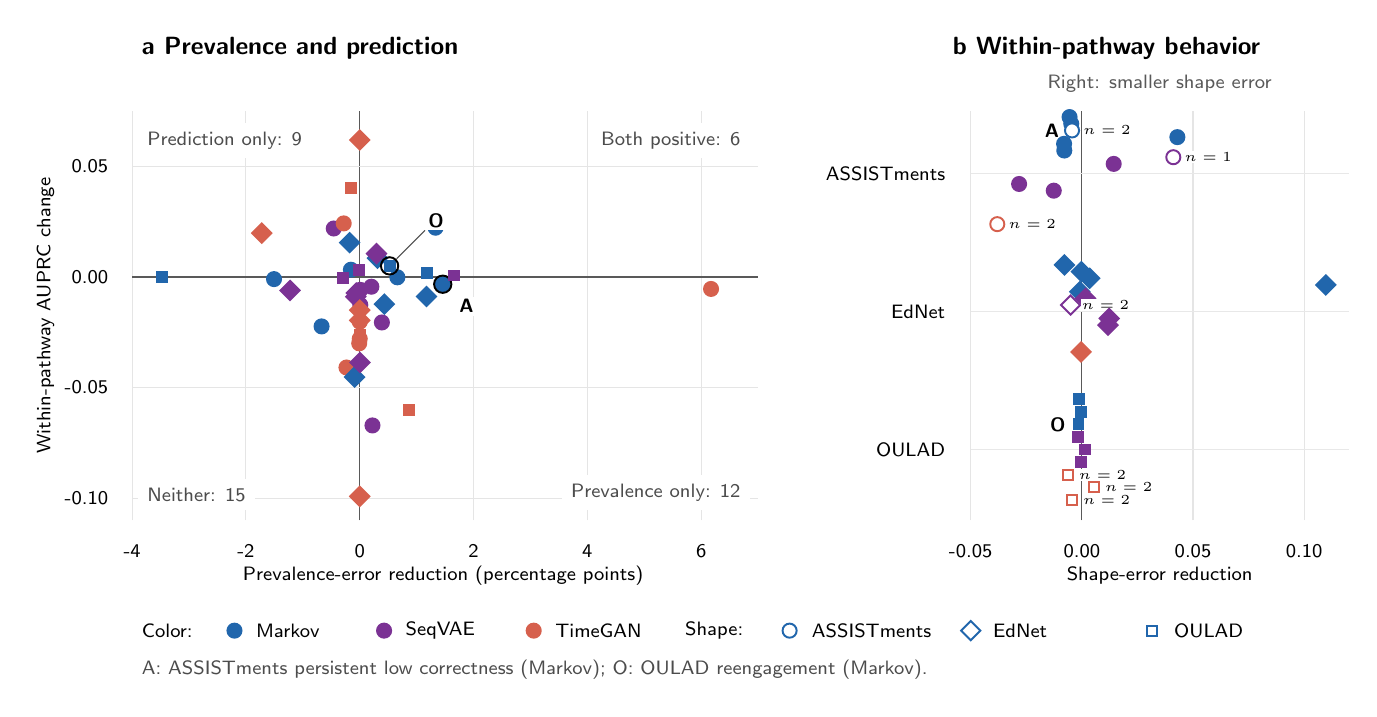
\begin{tikzpicture}[x=1cm,y=1cm,font=\sffamily]
\definecolor{paperblue}{HTML}{2166AC}
\definecolor{paperpurple}{HTML}{7B3294}
\definecolor{paperred}{HTML}{D6604D}
\node[font=\sffamily\scriptsize,anchor=west,font=\sffamily\bfseries\small] at (1.3500,7.1000) {a  Prevalence and prediction};
\node[font=\sffamily\scriptsize,anchor=west,font=\sffamily\bfseries\small] at (11.6500,7.1000) {b  Within-pathway behavior};
\draw[gray!20] (1.3500,1.1000) -- (1.3500,6.3000);
\node[font=\sffamily\scriptsize,anchor=north] at (1.3500,0.9100) {-4};
\draw[gray!20] (2.7955,1.1000) -- (2.7955,6.3000);
\node[font=\sffamily\scriptsize,anchor=north] at (2.7955,0.9100) {-2};
\draw[black!65] (4.2409,1.1000) -- (4.2409,6.3000);
\node[font=\sffamily\scriptsize,anchor=north] at (4.2409,0.9100) {0};
\draw[gray!20] (5.6864,1.1000) -- (5.6864,6.3000);
\node[font=\sffamily\scriptsize,anchor=north] at (5.6864,0.9100) {2};
\draw[gray!20] (7.1318,1.1000) -- (7.1318,6.3000);
\node[font=\sffamily\scriptsize,anchor=north] at (7.1318,0.9100) {4};
\draw[gray!20] (8.5773,1.1000) -- (8.5773,6.3000);
\node[font=\sffamily\scriptsize,anchor=north] at (8.5773,0.9100) {6};
\draw[gray!20] (1.3500,1.3811) -- (9.3000,1.3811);
\node[font=\sffamily\scriptsize,anchor=east] at (1.1700,1.3811) {-0.10};
\draw[gray!20] (1.3500,2.7865) -- (9.3000,2.7865);
\node[font=\sffamily\scriptsize,anchor=east] at (1.1700,2.7865) {-0.05};
\draw[black!65] (1.3500,4.1919) -- (9.3000,4.1919);
\node[font=\sffamily\scriptsize,anchor=east] at (1.1700,4.1919) {0.00};
\draw[gray!20] (1.3500,5.5973) -- (9.3000,5.5973);
\node[font=\sffamily\scriptsize,anchor=east] at (1.1700,5.5973) {0.05};
\node[font=\sffamily\scriptsize,rotate=90] at (0.2500,3.7000) {Within-pathway AUPRC change};
\node[font=\sffamily\scriptsize,] at (5.3000,0.4000) {Prevalence-error reduction (percentage points)};
\node[font=\sffamily\scriptsize,anchor=north west,text=black!70,fill=white] at (1.4200,6.1600) {Prediction only: 9};
\node[font=\sffamily\scriptsize,anchor=north east,text=black!70,fill=white] at (9.2000,6.1600) {Both positive: 6};
\node[font=\sffamily\scriptsize,anchor=south west,text=black!70,fill=white] at (1.4200,1.2200) {Neither: 15};
\node[font=\sffamily\scriptsize,anchor=south east,text=black!70,fill=white] at (9.2000,1.2200) {Prevalence only: 12};
\node[circle,draw=paperblue,fill=paperblue,line width=0.7pt,inner sep=1.8pt] at (5.2034,4.8171) {};
\node[circle,draw=paperblue,fill=paperblue,line width=0.7pt,inner sep=1.8pt] at (3.1519,4.1645) {};
\node[circle,draw=paperblue,fill=paperblue,line width=0.7pt,inner sep=1.8pt] at (5.2948,4.0997) {};
\draw[black,line width=.7pt] (5.2948,4.0997) circle (0.11);
\node[font=\sffamily\scriptsize,anchor=north west,font=\sffamily\bfseries\scriptsize,fill=white,inner sep=1pt] at (5.4648,3.9497) {A};
\node[circle,draw=paperblue,fill=paperblue,line width=0.7pt,inner sep=1.8pt] at (4.1285,4.2835) {};
\node[circle,draw=paperblue,fill=paperblue,line width=0.7pt,inner sep=1.8pt] at (4.7187,4.1873) {};
\node[circle,draw=paperblue,fill=paperblue,line width=0.7pt,inner sep=1.8pt] at (3.7561,3.5637) {};
\node[circle,draw=paperpurple,fill=paperpurple,line width=0.7pt,inner sep=1.8pt] at (4.3884,4.0678) {};
\node[circle,draw=paperpurple,fill=paperpurple,line width=0.7pt,inner sep=1.8pt] at (4.5219,3.6138) {};
\node[circle,draw=paperpurple,fill=paperpurple,line width=0.7pt,inner sep=1.8pt] at (4.2479,4.0281) {};
\node[circle,draw=paperpurple,fill=paperpurple,line width=0.7pt,inner sep=1.8pt] at (4.2479,3.8361) {};
\node[circle,draw=paperpurple,fill=paperpurple,line width=0.7pt,inner sep=1.8pt] at (3.9107,4.8071) {};
\node[circle,draw=paperpurple,fill=paperpurple,line width=0.7pt,inner sep=1.8pt] at (4.4025,2.3062) {};
\node[circle,draw=paperred,fill=paperred,line width=0.7pt,inner sep=1.8pt] at (4.2339,3.3489) {};
\node[circle,draw=paperred,fill=paperred,line width=0.7pt,inner sep=1.8pt] at (4.0723,3.0419) {};
\node[circle,draw=paperred,fill=paperred,line width=0.7pt,inner sep=1.8pt] at (4.2409,3.6226) {};
\node[circle,draw=paperred,fill=paperred,line width=0.7pt,inner sep=1.8pt] at (4.2409,3.4066) {};
\node[circle,draw=paperred,fill=paperred,line width=0.7pt,inner sep=1.8pt] at (8.7022,4.0395) {};
\node[circle,draw=paperred,fill=paperred,line width=0.7pt,inner sep=1.8pt] at (4.0372,4.8718) {};
\node[diamond,draw=paperblue,fill=paperblue,line width=0.7pt,inner sep=1.8pt] at (5.0885,3.9432) {};
\node[diamond,draw=paperblue,fill=paperblue,line width=0.7pt,inner sep=1.8pt] at (4.5537,3.8472) {};
\node[diamond,draw=paperblue,fill=paperblue,line width=0.7pt,inner sep=1.8pt] at (4.1127,4.6279) {};
\node[diamond,draw=paperblue,fill=paperblue,line width=0.7pt,inner sep=1.8pt] at (4.4661,4.4308) {};
\node[diamond,draw=paperblue,fill=paperblue,line width=0.7pt,inner sep=1.8pt] at (4.1752,2.9201) {};
\node[diamond,draw=paperpurple,fill=paperpurple,line width=0.7pt,inner sep=1.8pt] at (4.4536,4.4881) {};
\node[diamond,draw=paperpurple,fill=paperpurple,line width=0.7pt,inner sep=1.8pt] at (4.1971,3.9866) {};
\node[diamond,draw=paperpurple,fill=paperpurple,line width=0.7pt,inner sep=1.8pt] at (4.2440,3.1046) {};
\node[diamond,draw=paperpurple,fill=paperpurple,line width=0.7pt,inner sep=1.8pt] at (3.3558,4.0200) {};
\node[diamond,draw=paperpurple,fill=paperpurple,line width=0.7pt,inner sep=1.8pt] at (4.1909,3.9409) {};
\node[diamond,draw=paperred,fill=paperred,line width=0.7pt,inner sep=1.8pt] at (4.2409,1.4058) {};
\node[diamond,draw=paperred,fill=paperred,line width=0.7pt,inner sep=1.8pt] at (4.2409,3.7701) {};
\node[diamond,draw=paperred,fill=paperred,line width=0.7pt,inner sep=1.8pt] at (4.2409,3.6406) {};
\node[diamond,draw=paperred,fill=paperred,line width=0.7pt,inner sep=1.8pt] at (2.9962,4.7491) {};
\node[diamond,draw=paperred,fill=paperred,line width=0.7pt,inner sep=1.8pt] at (4.2409,5.9304) {};
\node[rectangle,draw=paperblue,fill=paperblue,line width=0.7pt,inner sep=1.8pt] at (5.0984,4.2422) {};
\node[rectangle,draw=paperblue,fill=paperblue,line width=0.7pt,inner sep=1.8pt] at (1.7322,4.1967) {};
\node[rectangle,draw=paperblue,fill=paperblue,line width=0.7pt,inner sep=1.8pt] at (4.6198,4.3325) {};
\node[rectangle,draw=paperpurple,fill=paperpurple,line width=0.7pt,inner sep=1.8pt] at (4.0247,4.1820) {};
\node[rectangle,draw=paperpurple,fill=paperpurple,line width=0.7pt,inner sep=1.8pt] at (5.4403,4.2101) {};
\node[rectangle,draw=paperpurple,fill=paperpurple,line width=0.7pt,inner sep=1.8pt] at (4.2317,4.2849) {};
\node[rectangle,draw=paperred,fill=paperred,line width=0.7pt,inner sep=1.8pt] at (4.8618,2.4976) {};
\node[rectangle,draw=paperred,fill=paperred,line width=0.7pt,inner sep=1.8pt] at (4.2391,3.4501) {};
\node[rectangle,draw=paperred,fill=paperred,line width=0.7pt,inner sep=1.8pt] at (4.1273,5.3253) {};
\draw[gray!20] (12.0000,1.1000) -- (12.0000,6.3000);
\node[font=\sffamily\scriptsize,anchor=north] at (12.0000,0.9100) {-0.05};
\draw[black!65] (13.4118,1.1000) -- (13.4118,6.3000);
\node[font=\sffamily\scriptsize,anchor=north] at (13.4118,0.9100) {0.00};
\draw[gray!20] (14.8235,1.1000) -- (14.8235,6.3000);
\node[font=\sffamily\scriptsize,anchor=north] at (14.8235,0.9100) {0.05};
\draw[gray!20] (16.2353,1.1000) -- (16.2353,6.3000);
\node[font=\sffamily\scriptsize,anchor=north] at (16.2353,0.9100) {0.10};
\node[font=\sffamily\scriptsize,anchor=east] at (11.8000,5.5000) {ASSISTments};
\draw[gray!18] (12.0000,5.5000) -- (16.8000,5.5000);
\node[font=\sffamily\scriptsize,anchor=east] at (11.8000,3.7500) {EdNet};
\draw[gray!18] (12.0000,3.7500) -- (16.8000,3.7500);
\node[font=\sffamily\scriptsize,anchor=east] at (11.8000,2.0000) {OULAD};
\draw[gray!18] (12.0000,2.0000) -- (16.8000,2.0000);
\node[font=\sffamily\scriptsize,] at (14.4000,0.4000) {Shape-error reduction};
\node[font=\sffamily\scriptsize,text=black!65] at (14.4000,6.6500) {Right: smaller shape error};
\node[circle,draw=paperblue,fill=paperblue,line width=.7pt,inner sep=1.8pt] at (13.2551,6.2225) {};
\node[circle,draw=paperblue,fill=paperblue,line width=.7pt,inner sep=1.8pt] at (13.2767,6.1375) {};
\node[circle,draw=paperblue,fill=white,line width=.7pt,inner sep=1.8pt] at (13.2867,6.0525) {};
\node[font=\sffamily\tiny,anchor=west,fill=white,inner sep=.5pt] at (13.4067,6.0525) {\(n=2\)};
\node[font=\sffamily\bfseries\scriptsize,anchor=east,fill=white,inner sep=.5pt] at (13.1467,6.0525) {A};
\node[circle,draw=paperblue,fill=paperblue,line width=.7pt,inner sep=1.8pt] at (14.6245,5.9675) {};
\node[circle,draw=paperblue,fill=paperblue,line width=.7pt,inner sep=1.8pt] at (13.1859,5.8825) {};
\node[circle,draw=paperblue,fill=paperblue,line width=.7pt,inner sep=1.8pt] at (13.1883,5.7975) {};
\node[circle,draw=paperpurple,fill=white,line width=.7pt,inner sep=1.8pt] at (14.5728,5.7125) {};
\node[font=\sffamily\tiny,anchor=west,fill=white,inner sep=.5pt] at (14.6928,5.7125) {\(n=1\)};
\node[circle,draw=paperpurple,fill=paperpurple,line width=.7pt,inner sep=1.8pt] at (13.8160,5.6275) {};
\node[circle,draw=paperpurple,fill=paperpurple,line width=.7pt,inner sep=1.8pt] at (12.6145,5.3725) {};
\node[circle,draw=paperpurple,fill=paperpurple,line width=.7pt,inner sep=1.8pt] at (13.0547,5.2875) {};
\node[circle,draw=paperred,fill=white,line width=.7pt,inner sep=1.8pt] at (12.3375,4.8625) {};
\node[font=\sffamily\tiny,anchor=west,fill=white,inner sep=.5pt] at (12.4575,4.8625) {\(n=2\)};
\node[diamond,draw=paperblue,fill=paperblue,line width=.7pt,inner sep=1.8pt] at (13.1902,4.3450) {};
\node[diamond,draw=paperblue,fill=paperblue,line width=.7pt,inner sep=1.8pt] at (13.4050,4.2600) {};
\node[diamond,draw=paperblue,fill=paperblue,line width=.7pt,inner sep=1.8pt] at (13.5109,4.1750) {};
\node[diamond,draw=paperblue,fill=paperblue,line width=.7pt,inner sep=1.8pt] at (16.5098,4.0900) {};
\node[diamond,draw=paperblue,fill=paperblue,line width=.7pt,inner sep=1.8pt] at (13.3850,4.0050) {};
\node[diamond,draw=paperpurple,fill=paperpurple,line width=.7pt,inner sep=1.8pt] at (13.4591,3.9200) {};
\node[diamond,draw=paperpurple,fill=white,line width=.7pt,inner sep=1.8pt] at (13.2682,3.8350) {};
\node[font=\sffamily\tiny,anchor=west,fill=white,inner sep=.5pt] at (13.3882,3.8350) {\(n=2\)};
\node[diamond,draw=paperpurple,fill=paperpurple,line width=.7pt,inner sep=1.8pt] at (13.7588,3.6650) {};
\node[diamond,draw=paperpurple,fill=paperpurple,line width=.7pt,inner sep=1.8pt] at (13.7431,3.5800) {};
\node[diamond,draw=paperred,fill=paperred,line width=.7pt,inner sep=1.8pt] at (13.4015,3.2400) {};
\node[rectangle,draw=paperblue,fill=paperblue,line width=.7pt,inner sep=1.8pt] at (13.3735,2.6400) {};
\node[rectangle,draw=paperblue,fill=paperblue,line width=.7pt,inner sep=1.8pt] at (13.3957,2.4800) {};
\node[rectangle,draw=paperblue,fill=paperblue,line width=.7pt,inner sep=1.8pt] at (13.3689,2.3200) {};
\node[font=\sffamily\bfseries\scriptsize,anchor=east,fill=white,inner sep=.5pt] at (13.2289,2.3200) {O};
\node[rectangle,draw=paperpurple,fill=paperpurple,line width=.7pt,inner sep=1.8pt] at (13.3607,2.1600) {};
\node[rectangle,draw=paperpurple,fill=paperpurple,line width=.7pt,inner sep=1.8pt] at (13.4477,2.0000) {};
\node[rectangle,draw=paperpurple,fill=paperpurple,line width=.7pt,inner sep=1.8pt] at (13.4055,1.8400) {};
\node[rectangle,draw=paperred,fill=white,line width=.7pt,inner sep=1.8pt] at (13.2301,1.6800) {};
\node[font=\sffamily\tiny,anchor=west,fill=white,inner sep=.5pt] at (13.3501,1.6800) {\(n=2\)};
\node[rectangle,draw=paperred,fill=white,line width=.7pt,inner sep=1.8pt] at (13.5623,1.5200) {};
\node[font=\sffamily\tiny,anchor=west,fill=white,inner sep=.5pt] at (13.6823,1.5200) {\(n=2\)};
\node[rectangle,draw=paperred,fill=white,line width=.7pt,inner sep=1.8pt] at (13.2816,1.3600) {};
\node[font=\sffamily\tiny,anchor=west,fill=white,inner sep=.5pt] at (13.4016,1.3600) {\(n=2\)};
\node[font=\sffamily\scriptsize,anchor=west] at (1.3500,-0.3000) {Color:};
\node[circle,draw=paperblue,fill=paperblue,line width=0.7pt,inner sep=1.8pt] at (2.6500,-0.3000) {};
\node[font=\sffamily\scriptsize,anchor=west] at (2.8000,-0.3000) {Markov};
\node[circle,draw=paperpurple,fill=paperpurple,line width=0.7pt,inner sep=1.8pt] at (4.5500,-0.3000) {};
\node[font=\sffamily\scriptsize,anchor=west] at (4.7000,-0.3000) {SeqVAE};
\node[circle,draw=paperred,fill=paperred,line width=0.7pt,inner sep=1.8pt] at (6.4500,-0.3000) {};
\node[font=\sffamily\scriptsize,anchor=west] at (6.6000,-0.3000) {TimeGAN};
\node[font=\sffamily\scriptsize,anchor=west] at (8.2500,-0.3000) {Shape:};
\node[circle,draw=paperblue,fill=white,line width=0.7pt,inner sep=1.8pt] at (9.7000,-0.3000) {};
\node[font=\sffamily\scriptsize,anchor=west] at (9.8600,-0.3000) {ASSISTments};
\node[diamond,draw=paperblue,fill=white,line width=0.7pt,inner sep=1.8pt] at (12.0000,-0.3000) {};
\node[font=\sffamily\scriptsize,anchor=west] at (12.1600,-0.3000) {EdNet};
\node[rectangle,draw=paperblue,fill=white,line width=0.7pt,inner sep=1.8pt] at (14.3000,-0.3000) {};
\node[font=\sffamily\scriptsize,anchor=west] at (14.4600,-0.3000) {OULAD};
\node[font=\sffamily\scriptsize,anchor=west,text=black!70] at (1.3500,-0.8000) {A: ASSISTments persistent low correctness (Markov); O: OULAD reengagement (Markov).};
\draw[black,line width=.7pt] (4.6198,4.3325) circle (0.11);
\draw[black!70,line width=.4pt] (4.7098,4.4225) -- (5.0698,4.7825);
\node[font=\sffamily\bfseries\scriptsize,anchor=south west,fill=white,inner sep=1pt] at (5.0698,4.7825) {O};
\end{tikzpicture}
}
\caption{Descriptive targeting effects. (a) Dataset--generator--pathway means: right indicates reduced prevalence error (standard minus targeted); up indicates higher within-pathway AUPRC (targeted minus standard). Quadrant counts use unrounded means. (b) Shape-error reduction requires at least ten qualifying real and synthetic learners per condition in a paired run. Hollow points label contributing counts below three; 12 summaries have no available paired mean. A and O mark the two examples discussed in the text.}
\label{fig:rq2-targeting-effects}
\end{figure}

\paragraph{Additional learner-level tasks.}
These tasks predict a later learner-level outcome, distinct from predicting the next response within a same-named whole-trajectory pathway. TimeGAN's synthetic-only persistent-low-correctness conditions contained only one outcome class in every tutoring-data seed, and most recovery comparisons also could not be calculated; the affected comparisons remain missing rather than being scored as zero. For ASSISTments persistent-low-correctness prediction, standard augmentation produced larger positive mean changes with Markov and SeqVAE, while TimeGAN's mean AUPRC change was close to zero (\(+0.0004\pm0.0154\); Supplementary Table~S12). These descriptive patterns did not establish a consistent benefit across tasks and settings. OULAD outcomes evaluate the complete processing procedure because dropout and failure are constructed after behavioral generation.

\subsection{Supporting Disclosure Audit}
\label{sec:disclosure-results}
No exact or threshold-defined near matches were found among evaluated ASSISTments or EdNet trajectories. Across standard and targeted tutoring conditions, mean membership-inference advantage ranged from 0.0000 to 0.0528; targeting increased the ASSISTments mean for all generators by 0.0178--0.0409. OULAD dominant-activity/engagement copying ranged from 0.31\% for standard SeqVAE to 15.57\% for standard TimeGAN. Supplementary Figure~S1 presents the detailed audit. These dataset-level findings neither estimate pathway-specific privacy nor certify release safety.
\FloatBarrier

\section{Discussion}

Synthetic learner pathways can occur at plausible rates without preserving the behavior or predictive information they represent. For RQ1, agreement on overall behavior did not reliably preserve event order or uncommon pathways. For RQ2, targeting sometimes improved pathway frequency without improving prediction for corresponding real learners, and sometimes the reverse occurred (Figure~\ref{fig:rq2-targeting-effects}). The Pathway-Centric Evaluation Lens therefore evaluates pathway frequency, behavior within the pathway, and prediction for real learners separately, according to the intended use.

\subsection{Temporal Fidelity and Behavioral Meaning}
\label{sec:window-assembly}

Matching response and activity rates did not establish event-order fidelity: recovery and decline can have the same correctness rate. Temporal learning-analytics research calls for aligning timing and order with the question being asked~\cite{knight2017time,molenaar2014sequential,saint2020combining}. Our findings extend that principle to generated records: required temporal properties must be checked directly, not inferred from aggregate similarity. Two trajectories can satisfy the same recovery rule yet differ between the early and late periods. Within-pathway checks therefore matter for claims about how recorded behavior develops. Prior work found that modeling cross-semester dependencies improved synthetic student pathways~\cite{huang2026pathways}. Here, Markov best preserved local-process measures, whereas SeqVAE more closely preserved early-to-late shape.

Overproducing the rare-skill pathway need not mean better coverage of uncommon behavior; generated records could make an unusual ordering appear widespread. Joining independently generated 20-event windows might create unlikely transitions: overproduction was largest in longer trajectories requiring several joins, while Markov used no joins and showed no comparable overproduction. We did not vary assembly, so this remains a hypothesis. Although TimeGAN was designed to preserve temporal dynamics~\cite{yoon2019timegan}, our findings concern the tested pipeline, including assembly and postprocessing, not TimeGAN generally.

\subsection{Pathway Frequency Is Not Predictive Usefulness}

In the ASSISTments Markov example, targeting brought persistent-low-correctness prevalence close to the real reference, but within-pathway AUPRC remained below the real-trained benchmark. The small standard-to-targeted difference does not establish harm; better prevalence agreement did not recover predictive usefulness. Qualifying trajectories may still lack the history--outcome relationships needed for prediction, but we did not isolate the cause.

Figure~\ref{fig:rq2-targeting-effects} also shows prediction gains without better prevalence fidelity. Descriptive research needs credible pathway frequencies, whereas predictor development may tolerate oversampling if performance improves on real learners. Thus, six joint gains among 42 descriptive comparisons are not a success rate for every use. This tradeoff resembles reported privacy--fairness--utility tensions~\cite{liu2025fairprivate}, but behavioral pathway representation is not demographic fairness.

\subsection{Prediction, Access, and Privacy Are Different Claims}

Our overall next-step losses contrast with near-real utility reported for some tabular learner-level tasks~\cite{liu2024scaling,khalil2025artificial}, but the studies differ in outcomes, generators, and evaluations. Poor real-data transfer for some models selected on synthetic validation data has also been reported~\cite{flanagan2022fine}; our findings extend that concern to pathway-specific evaluation. OULAD reengagement showed a pathway gain despite the overall loss, but the 19-enrollment test group cannot establish a general benefit.

Augmentation did not improve mean overall next-step AUPRC when real training data were available. Synthetic records might still support tool development under restricted access, with controlled real-data evaluation; we did not test that arrangement. Access value does not establish release safety. Targeting increased the dataset-level membership-inference signal in ASSISTments, consistent with cautions against assuming synthesis guarantees anonymity~\cite{stadler2022synthetic,vie2022privacy,vanbreugel2023membership}. Our audit provides neither a pathway-specific risk estimate nor a formal privacy guarantee.

\subsection{Implications for Use}

The lens extends resemblance, utility, and privacy assessments~\cite{liu2024scaling,liu2025ensuring} by linking fixed pathway definitions to prevalence, within-pathway behavior, and real-learner prediction. Synthetic fidelity and educational construct validity remain distinct: recovery and disengagement are operational groupings, not diagnoses of mastery, motivation, or self-regulation. In OULAD, nonzero clicks indicate platform activity, not cognitive or emotional engagement. Preserving an indicator does not validate a broader interpretation; distorting the indicator during synthesis further weakens that interpretation.

The checks inform decisions before use. Researchers estimating pathway frequencies need prevalence evidence; those studying behavioral development also need within-pathway temporal evidence. Developers need prediction tests on separate real learners, with pathway support counts. A failed or unavailable check calls for pipeline revision, further validation, or a narrower claim. Data stewards must assess disclosure separately. The lens sets no universal acceptance threshold and certifies no educational benefit. Prediction groups are defined retrospectively, so the scores show neither early identification of a pathway nor intervention benefit.

\subsection{Limitations}

The benchmark uses three datasets, three generators, three seeds, one learner split, one prespecified predictor, and one joint-targeting weighting scheme. Generator rankings and pathway-specific targeting effects may not transfer to other settings; predictive usefulness is conditional on the tested predictor. Small pathway groups limit precision. Event-level scoring gives longer trajectories more influence, so reported AUPRC is not an equal-weighted average across learners. OULAD resampling treats course enrollments as clusters rather than physical students, so uncertainty may not capture dependence between a student's enrollments. Shared OULAD outcome construction also limits generator-specific claims. Boundary diagnostics and a real-window assembly control could test the proposed explanation for inflated rare-skill counts. We assume benign source data and generation; adversarial manipulation requires separate integrity controls~\cite{liu2026quality}. The disclosure audit establishes neither pathway-specific safety nor differential privacy.

\section{Conclusion}

Reproducing a learner pathway's frequency did not ensure that synthetic trajectories preserved its behavior or supported prediction for corresponding real learners. Across three datasets and generators, overall resemblance did not consistently preserve temporal structure or uncommon pathways. Standard synthetic-only training lowered mean overall next-step AUPRC in all nine dataset--generator combinations; augmentation did not improve mean overall AUPRC. Targeting rarely improved pathway prevalence and prediction together.

The Pathway-Centric Evaluation Lens treats prevalence, within-pathway behavior, and real-learner prediction as separate validity checks for a stated use, not a universal generator ranking. Predictive usefulness does not establish privacy safety or improved educational outcomes.


\interlinepenalty=0
\bibliography{references}

\end{document}
